\documentclass[a4paper,12pt]{report}


%%%%%%%%%%%%%%%%%%%%%%%%%%%%
% University of Sussex thesis template
%%%%%%%%%%%%%%%%%%%%%%%%%%%%
% Modification History
%
% Based on usthesis.cls by Jonathon Read
% http://www.cogs.susx.ac.uk/users/jlr24/latex.html
% Modified by Anthony Smith, Feb 2007
% Incorporated into single thesis.tex file, Anthony Smith, 30 June 2008
% Minor alterations to page numbering, AJS, 25 July 2008
% New alternative hyperref options for print version, AJS, 11 Sep 2008
% "DRAFT" on header, AJS, 12 Sep 2008
%%%%%%%%%%%%%%%%%%%%%%%%%%%%


%%%%%%%%%%%%%%%%%%%%%%%%%%%%
% LINE SPACING 
\newcommand{\linespacing}{1.5}
\renewcommand{\baselinestretch}{\linespacing}
%%%%%%%%%%%%%%%%%%%%%%%%%%%%

%%%%%%%%%%%%%%%%%%%%%%%%%%%%
% CUSTOM COMMAND
\newcommand\ddfrac[2]{\frac{\displaystyle #1}{\displaystyle #2}}
%%%%%%%%%%%%%%%%%%%%%%%%%%%%

%%%%%%%%%%%%%%%%%%%%%%%%%%%%
% BIBLIOGRAPHY STYLE
\usepackage{natbib}
% \bibliographystyle{plain} for [1], [2] etc.
\bibliographystyle{apalike}
%%%%%%%%%%%%%%%%%%%%%%%%%%%%


%%%%%%%%%%%%%%%%%%%%%%%%%%%%
% OTHER FORMATTING/LAYOUT DECLARATIONS
% Graphics
\usepackage{graphicx,color}
\usepackage{epstopdf}
\usepackage[british]{babel}
\usepackage{threeparttable}  
\usepackage{caption}
\usepackage{subcaption}
\usepackage{float}
\usepackage{titlesec}
\usepackage{soul}
% The left-hand-side should be 40mm.  The top and bottom margins should be
% 25mm deep.  The right hand margin should be 20mm.
\usepackage[a4paper,top=3.5cm,bottom=3.5cm,left=4cm,right=3cm,headsep=10pt]{geometry}
\flushbottom
% Pages should be numbered consecutively thorugh the main text.  Page numbers
% should be located centrally at the top of the page.
\usepackage{fancyhdr}
\fancypagestyle{plain}{
	\fancyhf{}
	% Add "DRAFT: <today's date>" to header (comment out the following to remove)
	\lhead{\textit{DRAFT: \today}}
	%
	\chead{\thepage}
	\renewcommand{\headrulewidth}{0pt}
}
\pagestyle{plain}
%%%%%%%%%%%%%%%%%%%%%%%%%%%%


%%%%%%%%%%%%%%%%%%%%%%%%%%%%
% ANY OTHER DECLARATIONS HERE:
\titleformat*{\section}{\Large\bfseries}
%%%%%%%%%%%%%%%%%%%%%%%%%%%%


%%%%%%%%%%%%%%%%%%%%%%%%%%%%
% HYPERREF
\usepackage[colorlinks,pagebackref,pdfusetitle,urlcolor=blue,citecolor=blue,linkcolor=blue,bookmarksnumbered,plainpages=false]{hyperref}
% \usepackage{hyperref}
\usepackage{amssymb}
\usepackage{amsmath}
\usepackage{multirow}
% For print version, use this instead:
%\usepackage[pdfusetitle,bookmarksnumbered,plainpages=false]{hyperref}
%\usepackage{backref}
%\renewcommand{\backrefpagesname}{Cited on}
%%%%%%%%%%%%%%%%%%%%%%%%%%%%


%%%%%%%%%%%%%%%%%%%%%%%%%%%%
% BEGIN DOCUMENT
\begin{document}
%%%%%%%%%%%%%%%%%%%%%%%%%%%%


%%%%%%%%%%%%%%%%%%%%%%%%%%%%
% PREAMBLE: roman page numbering i, ii, iii, ...
\pagenumbering{roman}
%%%%%%%%%%%%%%%%%%%%%%%%%%%%


%%%%%%%%%%%%%%%%%%%%%%%%%%%%
%% TITLE PAGE: The title page should give the following information:
%%	(i) the full title of the thesis and the sub-title if any;
%%	(ii) the full name of the author;
%%	(iii) the qualification aimed for;
%%	(iv) the name of the University of Sussex;
%%	(v) the month and year of submission.
\thispagestyle{empty}
% \begin{flushright}
% 
\includegraphics[width=6cm]{uslogo}
% \end{flushright}	
\vskip40mm
\begin{center}
% TITLE
\huge\textbf{OOV Handling by Learning Subword using CNN based N-grams}\\
\vskip 1.5cm
% SUBTITLE (optional)
% \LARGE\textit{How it all works}
% \vskip5mm
% AUTHOR
\large Yonathan Purbo Santosa\\
Matriculation Number: 2993106\\
XXXX XX, XX\\
% \Large\textbf{Joe Bloggs}
% \normalsize
% \vfill
\vskip 1.5cm
Master thesis\\
Computer Science
% \vfill
\vskip 1.5cm
Supervisors:\\
Prof. Jehn Lehmann\\
Dr. Giulio Napolitano
\vfill
\textsc{Institut f{\"u}r Informatik III}\\
\textsc{Rheinische Friedrich-Wilhelms-Universit{\"a}t Bonn}
\end{center}
%%%%%%%%%%%%%%%%%%%%%%%%%%%%

\newpage
\thispagestyle{empty}
\mbox{}

%%%%%%%%%%%%%%%%%%%%%%%%%%%%
% DECLARATIONS
\chapter*{Declaration of Authorship}
I, Student name, declare that this thesis, titled "OOV Handling by
Learning Subword using CNN based N-grams", and the work presented in
it are my own. I confirm that:

\begin{itemize}
	\item This work was done wholly or mainly while in candidature for
	a research degree at this University.
	\item Where any part of this thesis has previously been submitted for a degree
	or any other qualication at this University or any other institution,
	this has been clearly stated.
	\item Where I have consulted the published work of others, this is always
	clearly attributed.
	\item Where I have quoted from the work of others, the source is always
	given. Except for such quotations, this thesis is entirely my own work.
	I have acknowledged all main sources of help.
	\item Where the thesis is based on work done by myself jointly with others,
	I have made clear exactly what was done by others and what I have
	contributed myself.
\end{itemize}
% ADDITIONAL DECLARATIONS HERE (IF ANY)

\vskip5mm
\underline{\makebox[0.9\linewidth][l]{Signed:}} \\~\\

\underline{\makebox[0.9\linewidth][l]{Date:}}

% AUTHOR
%%%%%%%%%%%%%%%%%%%%%%%%%%%%

%%%%%%%%%%%%%%%%%%%%%%%%%%%%
% ACKNOWLEDGEMENT
\chapter*{Acknowledgements}
blah blah blah
%%%%%%%%%%%%%%%%%%%%%%%%%%%%


%%%%%%%%%%%%%%%%%%%%%%%%%%%%
% SUMMARY PAGE
% \thispagestyle{empty}
% \newpage
% \null\vskip10mm
% \begin{center}
% \large
% \underline{UNIVERSITY OF SUSSEX}
% \vskip20mm
% % AUTHOR, QUALIFICATION
% \textsc{Joe Bloggs, Doctor of Philosophy}
% \vskip20mm
% % TITLE
% \underline{\textsc{My Theory of Everything}}
% \vskip0mm
% % SUBTITLE (optional)
% \underline{\textsc{How it all works}}
% \vskip20mm
% \underline{\textsc{Summary}}
% \vskip2mm
% \end{center}
% % Change line spacing
% \renewcommand{\baselinestretch}{1.0}
% \small\normalsize
% SUMMARY HERE (300 word limit for most subjects):

%%%%%%%%%%%%%%%%%%%%%%%%%%%%


%%%%%%%%%%%%%%%%%%%%%%%%%%%%
% TABLE OF CONTENTS, LISTS OF TABLES & FIGURES
\newpage
\pdfbookmark[0]{Contents}{contents_bookmark}
\tableofcontents
\listoftables
\phantomsection
\addcontentsline{toc}{chapter}{List of Tables}
\listoffigures
\phantomsection
\addcontentsline{toc}{chapter}{List of Figures}
%%%%%%%%%%%%%%%%%%%%%%%%%%%%


%%%%%%%%%%%%%%%%%%%%%%%%%%%%
% MAIN THESIS TEXT: arabic page numbering 1, 2, 3, ...
\newpage
\pagenumbering{arabic}
%%%%%%%%%%%%%%%%%%%%%%%%%%%%


%-----------------------------------------------------
% Chapter: Introduction
%-----------------------------------------------------

% NB Good idea to put each chapter in a separate file.
% If you put the following in a file called "thesis_introduction.tex"
% then you can include it with the following:

\chapter{Introduction}
\label{chap:intro}

% This is the introduction to the thesis.\footnote{And this is a
% footnote.}  The conclusion is in Chapter on page.
\section{Motivation} 
    Word embedding is a method for word representation mainly used in
    natural language processing domain. However, text data represented
    differently in machine unlike images and sounds data. Generally
    image is represented as two-dimensional to four-dimensional (given
    channels and alpha value) matrix with finite number of cell
    elements containing numerical value to represent color intensity
    on each location \citep{imageprocessing2018tyagi}. For example RGB
    image represented with 3-dimensional matrix. Each dimension
    represents the intensity of red color, green color, and blue color
    respectively in form of two-dimensional matrix. On the other hand,
    sound is represented as one-dimensional signal or stack of those
    signals (given several channels, it becomes two-dimensional)
    representing air pressure in the ear canal (for instance one
    channel for the left ear and one for the other)
    \citep{sound1995rocchesso}. Both images and sounds can be easily
    represented as mathematical models either using analog or digital
    signals but not with text data \citep{wordembedding2017yang}.
    Hence word embedding was introduced to give ability in
    representing text as a mathematical model namely a vector.
    
    Text data consists of sequence of characters that is represented
    by codes that is standardized, for example ASCII. In ASCII each
    character is represented by a number from $0$ to $127$ that later
    on extended until $255$. Combinations of these number then
    translated by computer to represent a character. Originally, in
    natural language processing text data can only be modeled using
    one-hot vector. This vector is a one-dimensional vector that has
    $d$-dimension, given \textit{d} words that are known or used. Each
    word is represented by one dimension and depends on the used word
    entries in the sentence, the correspondent dimension's value is
    $1$ and the rest is $0$ hence the name one-hot vector. The one-hot
    vector then stacked with another one-hot vectors to represent
    order of use in a sentence. Similar representation is also used to
    represent characters. The problem with one-hot vector is that it
    does not have any information that infers connection between one
    to another. It only encodes that certain word is used in a certain
    sentence in a certain sequence. Instead of sparse representation
    for each word, dense vector representations that maps semantic and
    syntactic information between words given one-hot vectors in a
    Euclidean space is introduced \citep{wordembedding2017yang,
    Distributed2013mikolov}. Hopefully, this positional information
    can be used to infer interconnection between words, whether its
    similarities or usage of the word in a sentence
    \citep{distributional1954harris}. To obtain word embeddings, a
    model is created to extract features of a word from a corpus and
    map its location in Euclidean space based on the features found
    \citep{Distributed2013mikolov, polyglot2013alrfou,
    dict2vect2017tissier}. These word embeddings then can be used to
    do many downstream tasks, such as POS-tagging, named entity
    recognition (NER), and sentiment analysis \citep{finding2015ling,
    neural2016lample}. 

    In general, large corpus with many words and examples of word
    usage is preferred because the size of the vocabularies will be
    higher and more words connection can be inferred from the corpus
    \citep{size2018kutuzov}. On top of that, multiple use of a
    vocabulary might also be used as a training data as an examples of
    cases of vocabulary usage in a sentence. However, it is not
    possible to have enough corpus since the language itself is
    creative and changing overtime \citep{forrester2008abrief,
    speech2009Jurafsky:2009:SLP:1214993}. Furthermore, there are cases
    of typographical error, especially on social media platform where
    anybody willingly write text over these platforms
    \citep{Liu2010SentimentAA} and some of these words may not be
    present in the corpus hence not included in the vocabulary even
    though there is another word that has the exact similar meaning to
    those words thus it should more or less has close distance to the
    standard or original word \citep{mapping2012eisenstein}. In
    addition with the increasing number of smartphones which uses
    touch screen, increase of number in typographical error is to be
    expected \citep{ghosh2017correction}. All these non-existent words
    in the corpus because of inability to collect such corpus or
    simply because of emergence of new slang or typographical error
    making the embedding of such word is unknown and it is called as
    \textit{out-of-vocabulary} (OOV) words. One may use simple
    approach by assigning unique random embedding for every OOV or by
    replacing OOV with an unknown \textit{\textless UNK\textgreater}
    token with randomly initialized embedding
    \citep{predicting2019garneau}, that later hoped to be generalized
    in training. Despite the fact that it can be used for OOV, further
    improvement on downstream tasks should be able to be achieved by
    using machine learning method to infer OOV embeddings.

    To infer OOV embeddings, the proposed model will be built over
    quasi-generative perspective. Only knowing the vocabularies and
    its embedding, the embedding for OOV words will be generated by
    the model. Previous \textit{state-of-the-art} used LSTM to infer
    OOV embeddings called \textsc{Mimick} \citep{mimicking2017Pinter}.
    For this model to infer OOV embedding, character embedding was
    first randomly initialized with a set of characters as its
    vocabulary. The character embedding then used to transform
    sequence of characters in a word into sequence of embedding. The
    sequence of the character embeddings then forwarded into
    bidirectional Long-Short Term Memory (bi-LSTM) then to fully
    connected layer. In language model, bi-LSTM generally works by
    separating sub-word by remembering and forgetting previous
    sequence from both end. How LSTM works in connection to this
    problem will be further explained in chapter \ref{chap:method}.
    The last hidden state of the bi-LSTM then will be used to infer
    its embedding. By architecture of LSTM, the gates inside the
    hidden neuron might drop previous information. Hence a problem
    might arise when there are more than two important sub-words and
    they are not in sequence, meaning that there exist at least one
    character between two sub-words considered important, hence the
    information is incomplete since the previous information will be
    dampened by LSTM hidden neuron interiors if the next sequence of
    sub-words are considered more important. This problem will be
    explained further in chapter \ref{chap:method}. From the
    explanation above, proposal of a new method to handle OOV is
    created.

\section{Objectives}
    For OOV to be inferred, a model that are able to generate
    embedding for the correspondence word has to be created. In
    \textsc{Mimick}, the whole sequence is processed by a bi-LSTM. By
    the problem mentioned earlier, instead of taking the whole words
    as a sequence and considering its importance based on time and
    occurrence using bi-LSTM, n-grams will be used to pick which grams
    (set of sequence) that are considered to be important. In theory
    this method should gives better results in downstream tasks since
    the information fed is complete and only left for the model to
    pick which n-grams features are more important. The only problem
    is that for the model to pick which grams that should be included
    in the model is impossible to do since there are many word
    combinations making the model needs to accept huge number of
    inputs. Instead of handpicking the features of n-grams,
    convolutional neural network (CNN) can be used to learn the
    existed features and pick which features needs to be considered by
    using character embedding and treat the character sequence
    embedding as two-dimensional matrix. The features picked then will
    be processed to predict the word embedding for the input word
    using feedforward network.

\section{Contributions}
    \begin{enumerate}
        \item An improved OOV handling model for downstream task
        \item Evaluation on different settings for baseline model and
        the proposed model
    \end{enumerate}

\section{Thesis Structure}
    The remainder of this document is structured as follows. In the
    \nameref{chap:relatedwork} chapter, the previous works that are in
    relatives with research done in this documents are mentioned
    especially the baseline used in this research. In the following,
    \nameref{chap:preliminaries} chapter, base theories for
    feedforward neural network, recurrent neural network, and n-grams
    that are considered to be needed are explained in details here. On
    top of that, the problem of the previous \textit{state-of-the-art}
    will be explained in depth here. In the \nameref{chap:method}
    chapter, the method of solution proposed to the problem and the
    testing method for analyzing the results are explained. In the
    \nameref{chap:implementation} chapter, the method of solution
    proposed to the problem are described in technical way to show how
    it is implemented and tested. In the \nameref{chap:results}
    chapter, the results are shown and discussed with the relation
    with the previous \textit{state-of-the-art}. Lastly,
    \nameref{chap:conc} chapter talks about the conclusion that are
    able to be pulled from this research.
\chapter{Related Work}
\label{chap:relatedwork}

% This is the introduction to the thesis.\footnote{And this is a
% footnote.}  The conclusion is in Chapter on page
Polyglot is one of word embeddings that is focused on multilingual
application \citep{polyglot2013alrfou}. A total of one hundred and
seventeen languages word embeddings were generated to give
availability of different language models to be trained. Previously,
specific language features were hand crafted by experts of specific
language \citep{polyglot2013alrfou}. This makes applying a language
model that are trained with commonly available language features
harder, hence the creation of Polyglot word embedding
\citep{polyglot2013alrfou}. This embedding was trained using Wikipedia
article and has no OOV handling if there exist a word that is not used
in Wikipedia. This pre-trained embedding was also used in the baseline
model \textsc{Mimick} for generating OOV embedding in many languages.

Word2vec is another word embedding that was trained using skip-gram
model \citep{efficient2013mikolov}. The available language choice for
this pre-trained embedding is English. A word $w(t)$ used as an input
and its context word, for example context word with windows of 4 are
$w(t-2), w(t-1), w(t+1),$ and $w(t+2)$ are used as the target. The model
tried to project the input $w(t)$ to the output to predict the context
words \citep{efficient2013mikolov}. Similar with Polyglot, this model
is highly dependent on the corpus completeness. The more examples and
vocabularies a corpus has, the better the representation of the
embeddings will be since more information will be able to be retrieved.
Word2vec model has no OOV handling either, meaning either random
vector or unknown ``\textit{\textless UNK\textgreater}'' embedding
will be used for it.

Dict2vec is yet another embedding that was trained by looking up
definitions of words from Cambridge dictionary
\citep{tissier2017dict2vec}. This embedding was created because the
previous method is trained with an unsupervised manner, which means that
there is no supervision between pairs of words. There might exists
a pair of words that are highly related but do not appear enough
inside a corpus which makes it harder for the model to find a connection
\citep{tissier2017dict2vec}. Thus, this model was trained by creating
sets of strong and weak pairs of words, then move both pairs closer
and further respectively based on the pairs. The model was evaluated by
using several word similarity tasks to show improvements over vanilla
implementation of word2vec and fasttext \citep{tissier2017dict2vec}.
Similar with previous word embedding, Dict2vec also has no OOV
handling method and since the vocabularies were only inferred from
Cambridge dictionary, there is no typographical error.

As aforementioned above, those word embedding has no way of handling
OOV words other than by assigning some unknown token
``\textit{\textless UNK\textgreater}'' or by letting the downstream
tasks model to train from the randomly generated embeddings each time
an OOV emerges. This case fueled \textsc{Mimick}, an OOV handling
model to be created \citep{mimicking2017Pinter}. This model was able
to tackle this problem successfully by using bi-directional long-short
term memory (bi-LSTM) to process embedding of characters of an OOV
word to produce the word embeddings. The OOV embedding generation
process was taken from quasi-generative perspective, which means that
the original embedding was assumed to has some form that could
generate the embeddings \citep{mimicking2017Pinter}. By doing so, the
OOV embeddings were able to be predicted without the needs of knowing
lexicon or model used for creating the word embedding. To prove that
such OOV handling model could perform better than randomly generated
embeddings or unique embedding for unknown token ``\textit{\textless
UNK\textgreater}'', several downstream tasks were used to evaluate the
model, such as Part-of-Speech-Tagging (POS-tagging) and word
similarity task that will be explained further below.

Part-of-Speech-Tagging (POS-tagging) is a process of determining
grammatical category called a \textit{tag} of a given word in a certain
sentence. In English, there are words that has ambiguous grammatical
category, such as word ``tag'' can either be noun or verb depending on
the usage of it \citep{apractical1992cutting}. To tackle this problem,
many researchers proposed to use of mathematical models or statistical
models namely hidden Markov model \citep{apractical1992cutting},
n-grams \citep{tnt2000Brants}, and neural network model
\citep{finding2015ling}. In this research, the neural network model
would be implemented to serve as the downstream task. This model was a
bi-LSTM that took sequence of word embeddings to represent a sentence
or parts of sentence then each word embedding were categorized for its
tag based on the usage in that sentence.

In spite of the performance of \textsc{Mimick}, there are evidence
of CNN that is used for sequence modeling can outperform LSTM and
RNN architecture \citep{empirical2018shaujie}. Moreover, CNN converges
faster than LSTM, RNN, and GRU based on the number of iteration
despite of the sequence length \citep{empirical2018shaujie}. The model
called temporal convolution network (TCN) is basically a multilayer
CNN with different dilation to factor the collection of input
dimension for each layer. The model was evaluated by using several
sequence modelling tasks.

For training an OOV model, some kind of feature extraction method
needs to be used. One of feature extraction method called n-grams is
often used to capture word features. N-grams can be applied in both
character grams in a word or word grams in a sentence. With character
embedding and convolution neural network (CNN), n-grams can be
calculated by convoluting sets of characters embedding with the kernel
size of $n \times d$ for $n$ is the number of grams and $d$ is the
dimension of the embeddings. This CNN n-grams then can be used to
create a neural language model \citep{character2015kim}.

\cite{character2015kim} created a language model for several
languages. This model used character n-grams by using character
embeddings and processed with CNN like an image. The results from
these process then passed through a highway network. A highway network
controls whether the information from the input would also be carried
to the next process or to be changed with original embedding or ASCII
code. The output of the highway network then passed through LSTM to
predict the next word. In those research, the results of the model for
OOV nearest neighbor trained with or without highway network were
compared. The results was that the one trained without highway network
has closer distance to a word that has smallest edits while the one
that trained with the highway network has closer distance to a word
with similar orthographic \citep{character2015kim}.

\cite{batchnorm:DBLP:journals/corr/IoffeS15} proposed a model to
compensate slower training time caused by internal covariate shift.
This phenomenon happened because the distribution of values changes
between layers in neural network, making training model that saturates
to a nonlinearity activation function harder
\citep{batchnorm:DBLP:journals/corr/IoffeS15}. By using a method
called Batch Normalization, each layer's inputs were normalized to
match distribution of certain mean and variance. As a result, larger
learning rates can be used and smaller training epoch was needed to
achieve a certain error values compared to the one without Batch
Normalization \citep{batchnorm:DBLP:journals/corr/IoffeS15}.
\chapter{Preliminaries}
\label{chap:preliminaries}

\section{Feedforward Neural Network}
    Feedforward neural network or also known as multilayer perceptron
    (MLP) are a mathematical model that is inspired from how neuron
    works in biological body \citep{Goodfellow-et-al-2016}. The model
    takes numerical input as a stimulus and produces numerical output
    as a response. This model is a simplification of animal nervous
    system. Originally, it was a single layer of input and a single
    layer of output. The cells within input layer and output layer is
    called neuron. Those neurons are responsible for the numerical
    representation of the input and the output. Given an input vector
    $\mathbf{x_i}$ with $n$-dimension from a dataset $D =
    \{(\mathbf{x_1}, y_1), (\mathbf{x_2}, y_2), \dots, (\mathbf{x_i},
    y_i)\}$, the model tries to predict a target $y_i$ correctly given
    a set of weights $\mathbf{w}$. The weights act as stimulus
    intensity value, thus different weight values will produces
    different responses given similar input stimulus and so is
    different responses given different input stimulus with similar
    weight values. The output $o_i$ is calculated by using the dot
    product between $\mathbf{x_i}$ and $\mathbf{w}$ as follows, 
    \begin{align}
        \label{eq:perceptron_out}
        o_i &= \mathbf{x_i} \cdot \mathbf{w} \\
        o_i &= \sum_{j=1}^n (x_{ij} \times w_j)
    \end{align}
    After calculating the output $o_i$ and another parameter bias $b$
    is added, the result is passed to activation function $f(o_i)$ to
    produce the model output $\hat{y_i}$ as follows,
    \begin{equation}
        \label{eq:perceptron_act}
        f(o_i) = \hat{y_i} =
        \begin{cases}
            1 & \text{if }\ o_i + b > 0,\\
            0 & \text{otherwise}
        \end{cases}
    \end{equation}
    This model is called perceptron and it is depicted in figure
    \ref{fig:perceptron}. The input information is fed through the model
    in chain with no feedback thus the name feedforward
    \citep{Goodfellow-et-al-2016}. When the outputs are fed back into
    the model, the model becomes recurrent network and it will be
    explained in the next subchapter.

    \begin{figure}
        \centering
        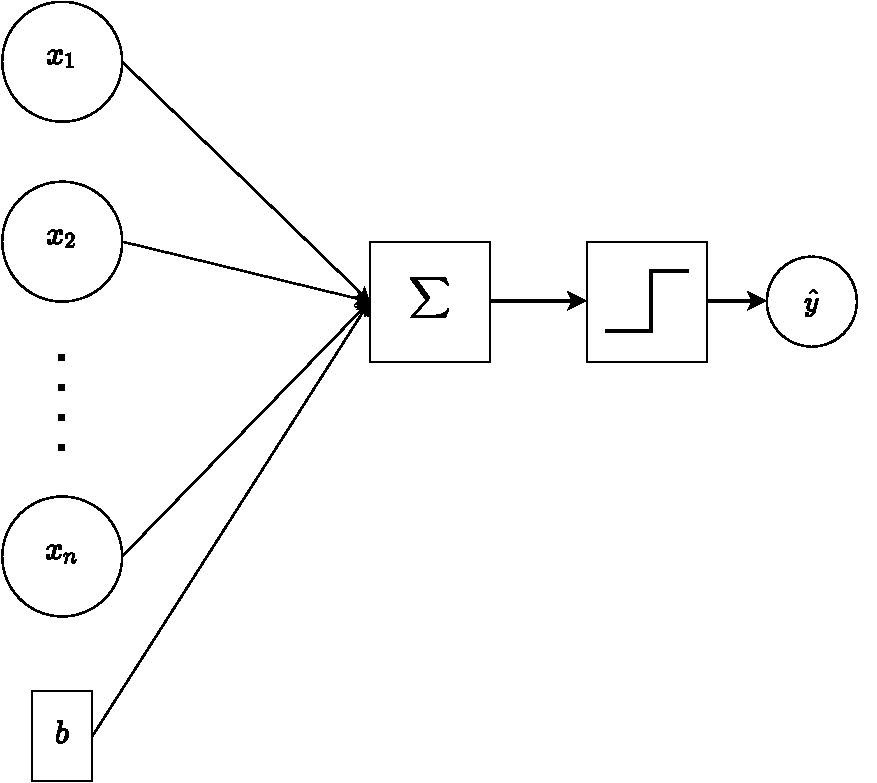
\includegraphics[width=.5\linewidth]{images/perceptron.pdf}
        \caption{Perceptron}
        \label{fig:perceptron}
    \end{figure}
    
    The results then compared with the target output $y_i$ in the
    dataset to learn the correct parameter weight $\mathbf{w}$ and
    bias $b$ by using backpropagation algorithm. The algorithm defines
    a cost function and calculate the gradient based on the current
    cost, then the gradient information is processed by another
    algorithm called stochastic gradient descent to try to find the
    optimal parameters that are producing the minimum cost. If
    $\mathbf{\hat{y}} = f(\mathbf{x}, \mathbf{W}) = \mathbf{x} \cdot
    \mathbf{W}$ and the cost $z = J(\mathbf{y})$, the simple
    calculation of the gradient can be calculated as follows,
    \begin{align}
        \label{eq:gradient1}
        \frac{\partial z}{\partial x_i} &= \sum_j \frac{\partial z}{\partial y_j} \frac{\partial y_j}{\partial x_i}\\
        \label{eq:gradient2}        
        &= \sum_j \frac{\partial z}{\partial y_j} \sum_k w_k
    \end{align}
    The correction on parameter $\mathbf{W}$ can be calculated with
    some learning parameter $\eta$ as shown on equation \ref{eq:sgd}.
    \begin{align}
        \label{eq:sgd}
        \hat{w_i} = -\frac{\partial z}{\partial x_i} \times \eta \times w_i
    \end{align}
    Notice that the gradient in equation \ref{eq:sgd} is multiplied by
    $-1$ because the gradient points uphill and to find the minimum
    cost, the parameters needs to traverse downhill on the cost
    function. The learning parameter $\eta$ act as penalization factor
    for the gradient to avoid jumping over the optimal solution.
    Generally, $\eta$ is set to be near zero.
    
    On the development of perceptron, it is clear that model
    consisting of single layer of input and single layer of output
    does not enough to solve XOR problem
    \citep{Goodfellow-et-al-2016}, since what perceptron does is
    separating the space with a hyperplane, or in XOR problem a
    hyperline as shown on figure \ref{fig:xor}. 
    \begin{figure}
        \centering
        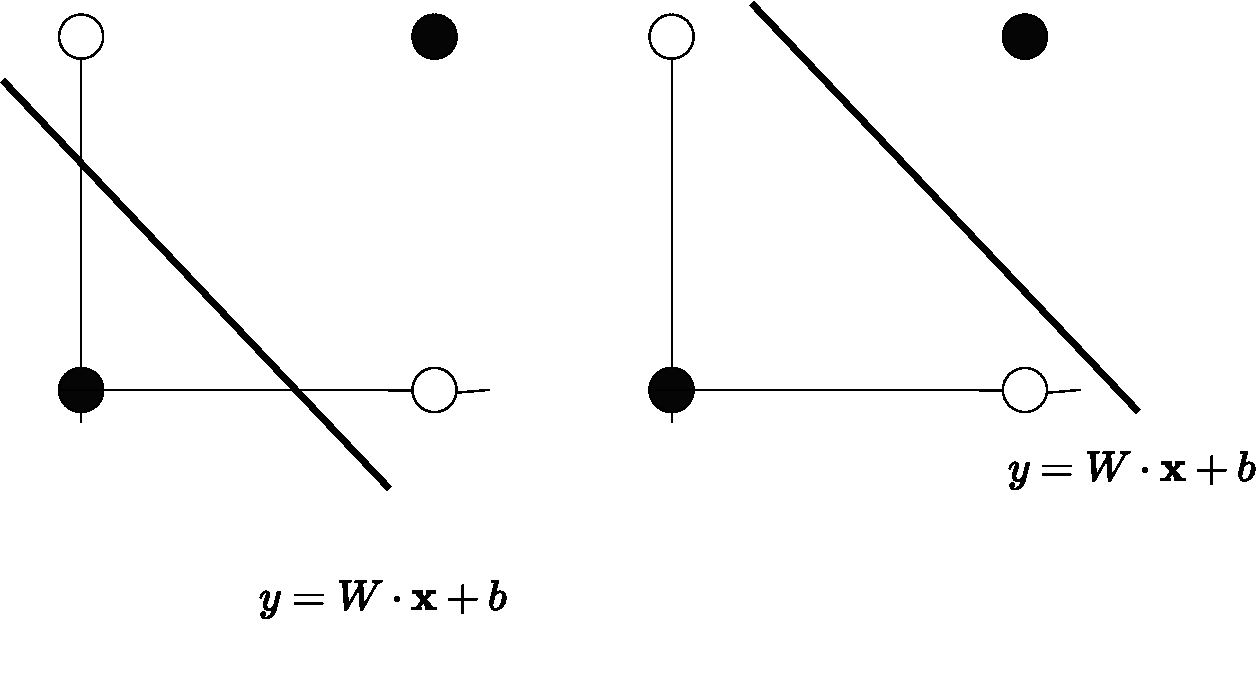
\includegraphics[width=.7\linewidth]{images/xor.pdf}
        \caption{XOR Problem}
        \label{fig:xor}
    \end{figure}
    Thus multilayer perceptron were introduced. This model consist of
    single layer of input, single layer of output, and one or more
    hidden layer. On top of that, more non-linear activation function
    were introduced. Some of those are sigmoid, tanh, rectified linear
    unit (ReLU), and softmax described in equation \ref{eq:sigmoid}
    until \ref{eq:softmax}. This nonlinearity makes the model easier
    to train since those functions are differentiable.

    \begin{align}
        \label{eq:sigmoid}
        \sigma(x) &= \frac{1}{1+e^{-x}} \\
        \label{eq:tanh}
        tanh(x) &= \frac{e^x-e^{-x}}{e^x + e^{-x}}\\
        \label{eq:relu}
        ReLU(x) &= x^+ = max(0, x)\\
        \label{eq:softmax}
        softmax(x) &= \frac{e^{x_i}}{\sum_{j=1}^J e^{x_j}}
    \end{align}

\section{Long-short Term Memory}
    \begin{figure}[H]
        \centering
        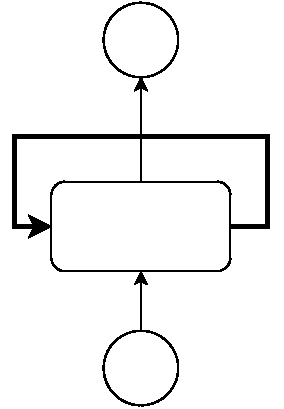
\includegraphics[width=.15\linewidth]{images/rnn.pdf}
        \caption{Recurrent Neural Network}
        \label{fig:rnn}
    \end{figure}
    \begin{figure}[H]
        \centering
        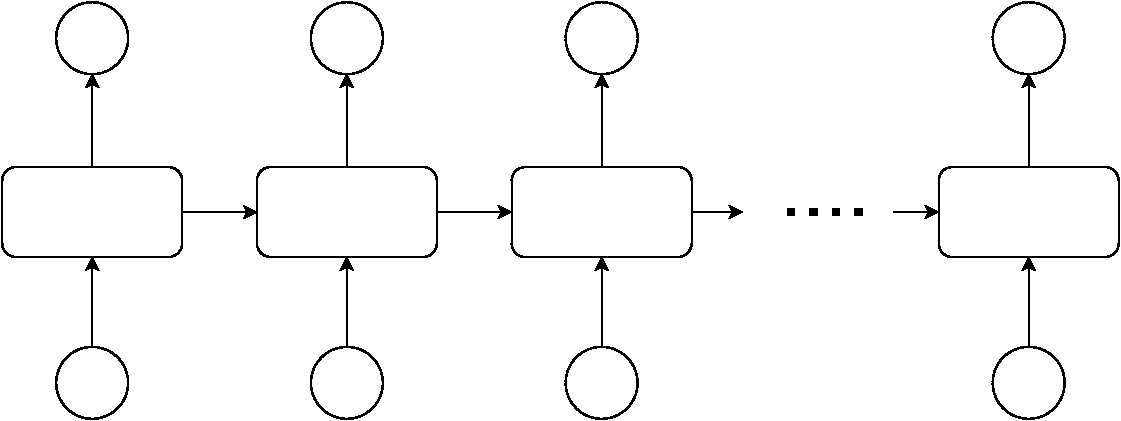
\includegraphics[width=.6\linewidth]{images/unfolded_rnn.pdf}
        \caption{Unfolded Recurrent Neural Network}
        \label{fig:unfolded_rnn}
    \end{figure}
    As previously mentioned, recurrent neural network (RNN) is a
    neural network model that has feedback to its own neuron depicted
    in figure \ref{fig:rnn}. This model used for processing sequential
    data \citep{Goodfellow-et-al-2016}. The idea is given sequence of
    input with length of $t$, $\mathbf{x}_i^{(t)} = x_i^{(1)}, x_i^{(2)},
    \dots, x_i^{(\tau)}$, the input is processed with shared parameter to
    give $t$-lengths output as depicted in figure
    \ref{fig:unfolded_rnn}. Common usage of RNN is for processing
    sentence. For example, given two sentences "I went to Paris in
    2004" and "In 2004 I went to Paris". If we query the model to
    extract information from both sentences and ask when did the
    narrator went to Paris, 2004 would be the relevant information
    regardless when it is appears in a sentence
    \citep{Goodfellow-et-al-2016}. If such task is trained using a
    feedforward neural network that processes fixed size inputs, the
    parameters for each input feature will be separated for each
    sequence. In comparison with feedforward neural network, RNN will
    use the same parameters to process all of the input sequence. 

    The problem with RNN is that when given a really long sequence,
    either the gradient calculation will vanish since if weight is
    near zero and it is multiplied several times sequentially over
    time and the gradient exploded if the weight is larger than one
    and it is multiplied several times \citep{Goodfellow-et-al-2016}.
    Those problems making processing long sequence on RNN unfavorable.
    Hence another method called long-short term memory (LSTM) was
    introduced. LSTM was created with idea in mind that some paths
    exist to give gradient ability to flow for long sequence
    \citep{Goodfellow-et-al-2016}. This was achieved by introducing
    self-loops inside the hidden layer that has time-scale mechanism
    that can change dynamically based on the input and previous state
    \citep{Goodfellow-et-al-2016}. New components called cell gate
    $C_t$, forget gate $f_t$, and input gate $i_t$ are introduced to
    let the recurrent network split the graph of the hidden unit thus
    gradient can be flowed longer by depending only from the output
    $o_t$ or from both output and hidden states $o_t$ and $h_t$
    respectively. The calculation process of LSTM for each time step
    $t=1$ to $t=\tau$ is as follows,
    \begin{align}
        \label{eq:lstm:f_t}
        f_t &= \sigma(W_f \cdot [h_{t-1}, x_t] + b_f) \\
        \label{eq:lstm:i_t}    
        i_t &= \sigma(W_i \cdot [h_{t-1}, x_t] + b_i) \\
        \label{eq:lstm:Cc_t}
        \tilde{C}_t &= tanh(W_C \cdot [h_{t-1}, x_t] + b_C) \\
        \label{eq:lstm:C_t}
        C_t &= f_t \times C_{t-1} + i_t \times \tilde{C}_t \\
        \label{eq:lstm:o_t}
        o_t &= \sigma(W_o \cdot [h_{t-1}, x_t] + b_o) \\
        \label{eq:lstm:h_t}
        h_t &= o_t \times tanh(C_t) \\
        \label{eq:lstm:y_t}
        \hat{y_t} &= softmax(o_t)
    \end{align}
    The forget gate $f_t$ and the input gate $i_t$ interacts with
    input $x_t$, previous hidden state $h_{t-1}$, and previous cell
    gate $C_{t-1}$ to control the current cell gate $C_t$. This cell
    gate $C_t$ will be used to control the information flow from
    previous hidden state $h_{t-1}$ to the current hidden state $h_t$
    as shown in equation \ref{eq:lstm:h_t}. If $C_t = 0$, the hidden
    state $h_t$ will be $0$, meaning the previous information of a
    certain features is dropped for the gated hidden states. The LSTM
    hidden cell's architecture is depicted in figure \ref{fig:lstm}.

    On top of the normal sequence, the reverse sequence can also be
    calculated starting at time step $t=\tau$ to $t = 1$ then the
    output is joined with the forward sequence. This method is called
    bidirectional-LSTM (bi-LSTM) depicted in figure \ref{fig:bilstm}.
    
    \begin{figure}
        \centering
        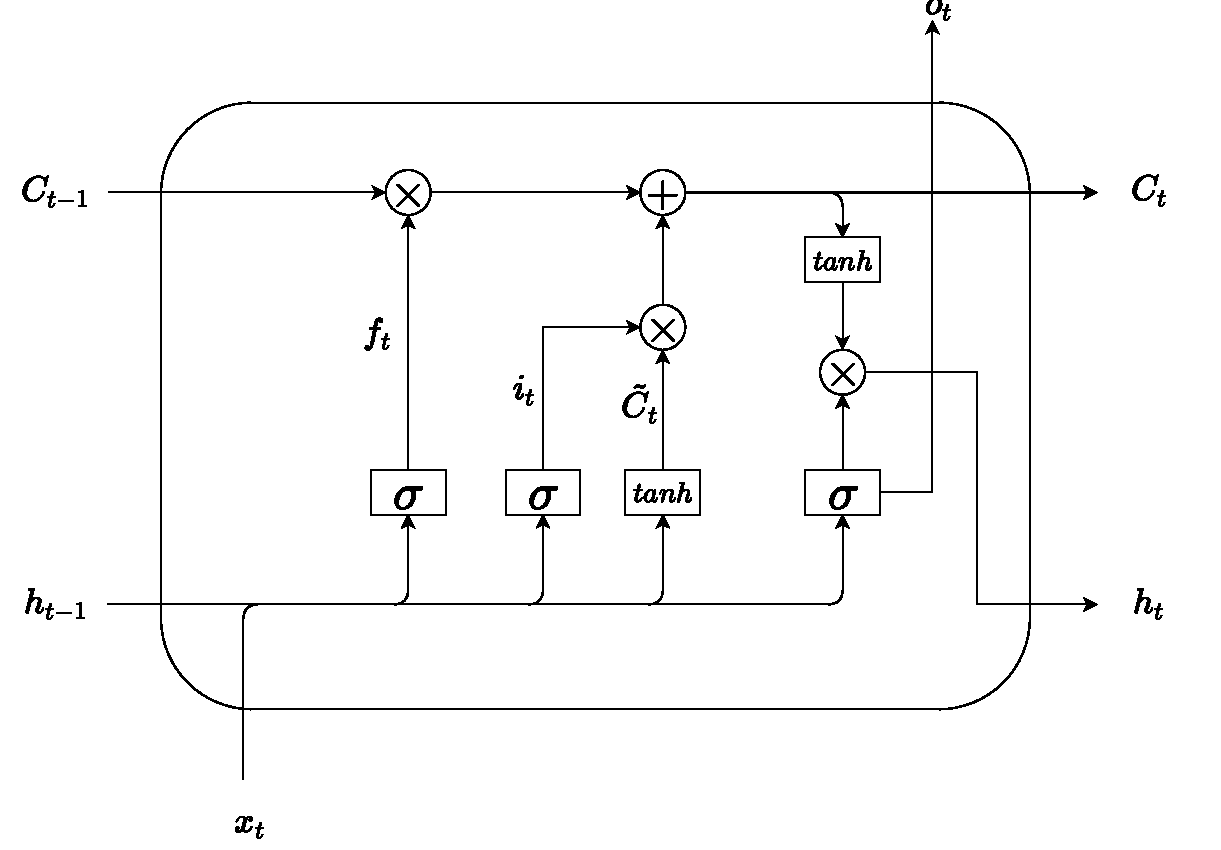
\includegraphics[width=.6\linewidth]{images/lstm.pdf}
        \caption{Gates inside LSTM hidden cell}
        \label{fig:lstm}
    \end{figure}

    \begin{figure}[H]
        \centering
        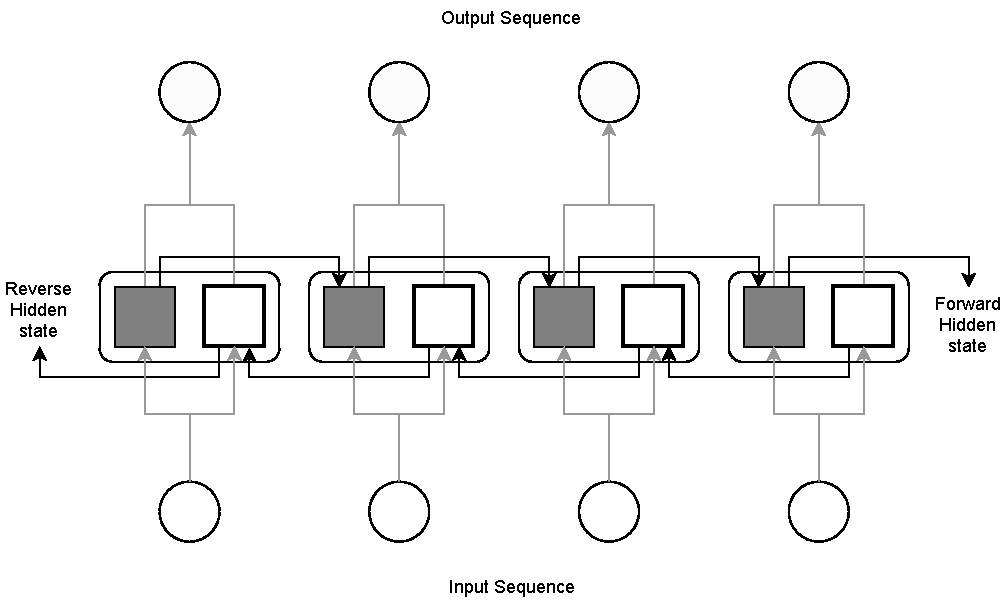
\includegraphics[width=.8\linewidth]{images/bi-lstm.pdf}
        \caption{bi-LSTM with 4 sequence}
        \label{fig:bilstm}
    \end{figure}

\section{Mimick}
    In this research, \textsc{Mimick} is used as baseline model.
    Firstly, pre-trained embedding which contains word $w_i$ and its
    embedding $e_i$ is used as input and target respectively.
    Afterward, the character embedding $g_i \in \mathbf{G}$ for each
    character $c_i \in \mathbf{C}$ was defined. Each word $w_i$ as
    input first broken down into sequence of characters, $w_i = [c_1,
    c_2, \dots, c_n]$, then each character was transformed into its
    embedding, producing sequence of character embeddings $[g_1, g_2,
    \dots, g_n]$. Those character embeddings then fed into bi-LSTM as
    a sequence to extract the features of the word input. The last
    hidden states of both forward $\mathbf{h}_f$ and backward
    $\mathbf{h}_b$ then concatenated and fed into a fully connected
    layer with parameters $\mathbf{T}_h$, $\mathbf{b}_H$,
    $\mathbf{b}_T$ and $\mathbf{O}_T$ and nonlinear function $g$ to
    predict the embedding of the input word as described by equation
    \ref{eq:mimick}.
    \begin{equation}
        \label{eq:mimick}
        f(w) = \mathbf{O}_{T} \cdot g(\mathbf{T}_h \dot [\mathbf{h}_f;
        \mathbf{h}_b] + \mathbf{b}_h) + b_T
    \end{equation}
    The objective of the training is to get the predicted embedding
    $f(w_i)$ as close as the pre-trained word embeddings $e_i$. This
    was done by minimizing the squared Euclidean error,
    \begin{equation}
        \label{eq:mimickloss}
        \mathcal{L} = \Vert f(w_i) - e_i \Vert_2^2
    \end{equation}
    The full process of predicting the embedding $f(w_i)$ is depicted
    in figure \ref{fig:mimick}.
    \begin{figure}
        \centering
        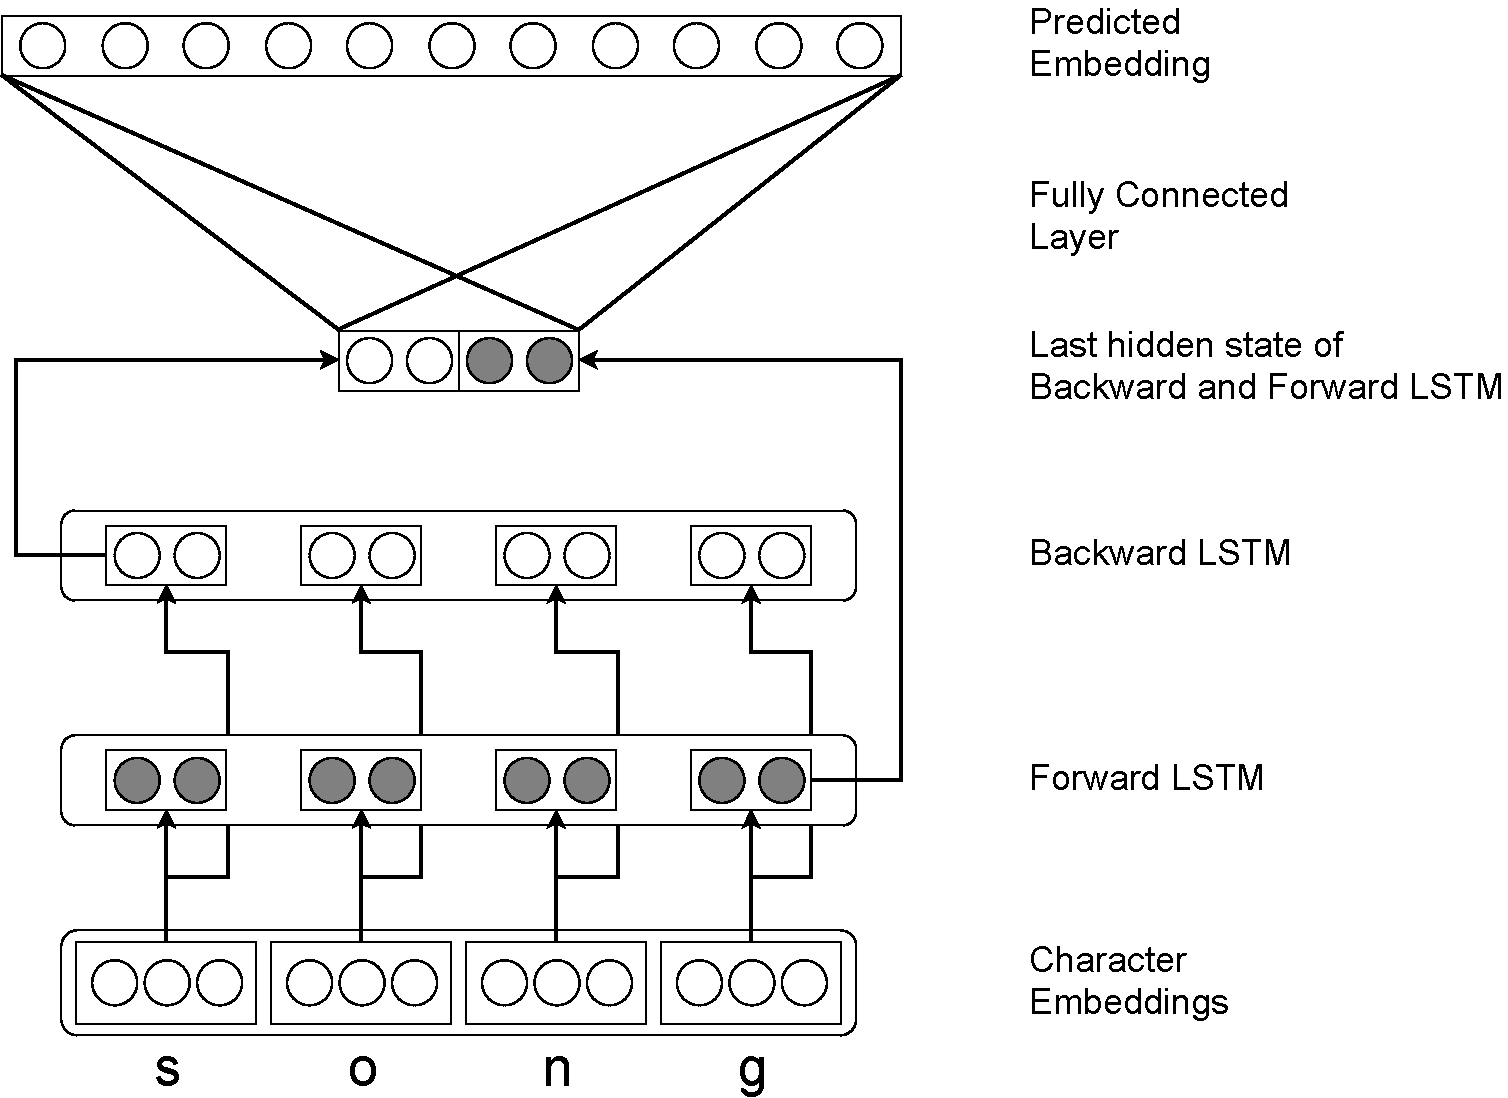
\includegraphics[width=.8\linewidth]{images/mimick.pdf}
        \caption{Mimick architecture}
        \label{fig:mimick}
    \end{figure}

    As already indicated in the previous subchapter, cell gate $C_t$
    controls which hidden neuron in hidden states at time $t$ will
    pass through to the next sequence. \textsc{Mimick} uses only the
    last hidden state of the bi-LSTM thus increases the chance of the
    early important sequence to be dropped when cell gate $C_t$
    decided to drop the information at certain point when there exist
    some input vector $\hat{x}_t$ or hidden state $\hat{h}_{t-1}$ that
    could trigger the cell gate $C_t$ to drop previous information
    entirely. Although bi-LSTM could serve the purpose to include the
    early sequence, there might exist intermediate sequence that
    appears in the middle of two important sequences that could be
    dropped because of the cell gate $C_t$ decided to drop previous
    sequence for both forward and reverse LSTM. The solution to this
    is to increase the number of hidden states size to reduce such
    chance. 
    
    This problem fueled another approach to be introduced, namely
    using convolutional neural network (CNN) as the feature extractor
    for the character sequence. 

\section{Convolutional Neural Network}
    Convolutional neural network (CNN) is a model that is used to
    process data that has grid topology \citep{Goodfellow-et-al-2016}.
    For a time series data that has a regular time interval, CNN can
    process this as a one-dimensional grid data and for an image data
    CNN can process this as a two-dimensional grid or 3-dimensional
    grid given the number of channel presents on the image data. This
    model concept was first introduced for handwriting recognition
    \citep{generalization1989lecun}.

    In general, convolution is operation of two function, the data and
    the kernel, that is taking values from both function and
    element wise multiplied was done and then summed to get the total
    overlaps between both function at time $t$. In general, the kernel
    has only limited size that has non-zero values while the rest is
    zero. Thus the convolution operation is done locally by processing
    parts of the data several times. To obtain the entirety processed
    data, the kernel needed to be shifted in all direction depending
    on the data dimension. This process is easier to be explained with
    mathematical expression. In equation \ref{eq:conv:2},
    one-dimensional data or function $f(t)$ is being convoluted with a
    kernel $g(t)$.
    \begin{align}
        \label{eq:conv:1}
        h(t) &= (f * g)(t)\\
        \label{eq:conv:2}
        h(t) &= \int_{-\infty}^\infty f(u)g(t-u) du
    \end{align}
    In discrete type signal, the calculation processes becomes as
    shown in equation \ref{eq:conv_d:2}.
    \begin{align}
        \label{eq:conv_d:1}
        h(t) &= (f * g)(t)\\
        \label{eq:conv_d:2}
        h(t) &= \sum_{u = -\infty}^{\infty} f(u)g(t-u)
    \end{align}
    For two-dimensional data, the discrete convolution function
    becomes as shown in equation \ref{eq:conv_d_2d}.
    \begin{align}
        \label{eq:conv_d_2d}
        h[i, j] = \sum_{m = -\infty}^{\infty}\sum_{n = -\infty}^{\infty}f[m, n]\cdot g[i-m, j-n]
    \end{align}

    In CNN, one of the function is the input data and the other is the
    weight. Typically, the weight's, also known as kernel, size is
    smaller than the input data although it is possible to have kernel
    size that is bigger than the input but there is no reason to have
    larger kernel if the objective is to learn local features of the
    data. To process an image data, the image input is convoluted with
    some kernels to produce different spatial features. This features
    then will be processed with a feedforward neural network to
    produce some prediction of classification or regression. The
    convolution process of one patch of an input image is depicted in
    figure \ref{fig:convolution}.
    
    \begin{figure}
        \centering
        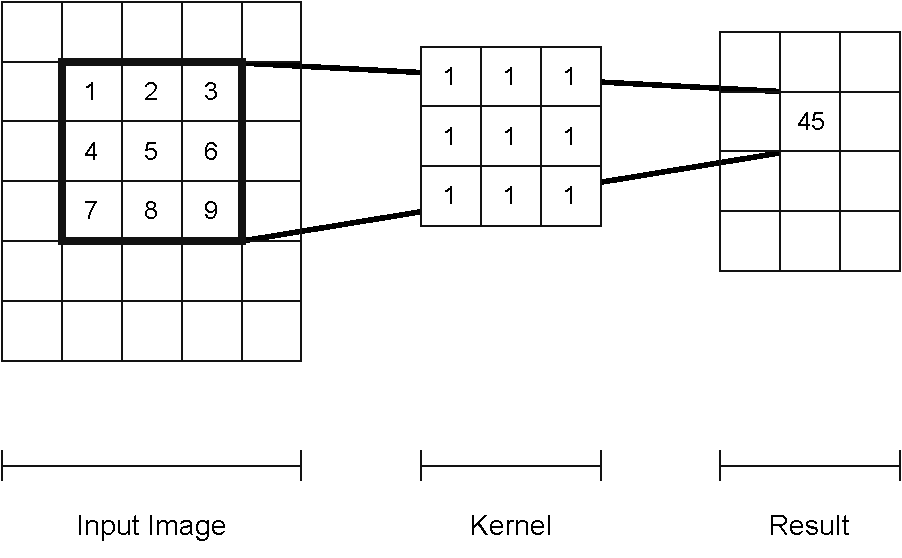
\includegraphics[width=.6\linewidth]{images/convolution.pdf}
        \caption{Convolution process of input image with kernel size $3\times3$}
        \label{fig:convolution}
    \end{figure}
    
    Another intermediate layer that can also be used in CNN called
    maxpooling layer. Maxpooling is a process of finding a maximum
    value inside a given window from a given grid. In CNN, maxpooling
    is used for finding within the input data that gives the highest
    response with a given kernel. Then the process of convolution and
    maxpooling is repeated until desired architecture is produced. The
    process of one patch of an input image is depicted in figure
    \ref{fig:maxpool}. Maxpooling process act as a gate for the
    highest response to receive backward connection for correcting the
    kernel. This is so that only parts of the image that has highest
    response will also corresponds to the correction of the kernel
    while the others treated as less useful. 

    \begin{figure}
        \centering
        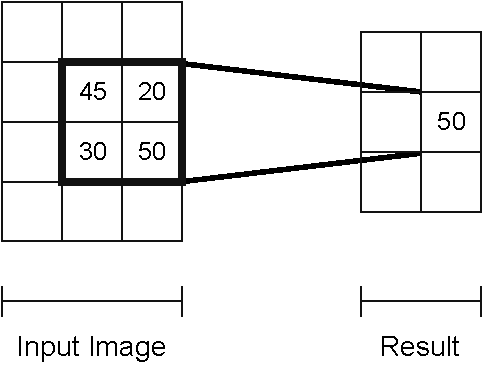
\includegraphics[width=.4\linewidth]{images/maxpool.pdf}
        \caption{Maxpooling process of input image with window size $2\times2$}
        \label{fig:maxpool}
    \end{figure}

    Convolution and maxpool then can be combined together to produce
    features map that act as input to the fully connected network. As
    an example, CNN with two convolution and maxpool architecture is
    depicted in figure \ref{fig:cnn}. In most cases, after doing
    convolution, non-linear activation function are applied.
    
    \begin{figure}
        \centering
        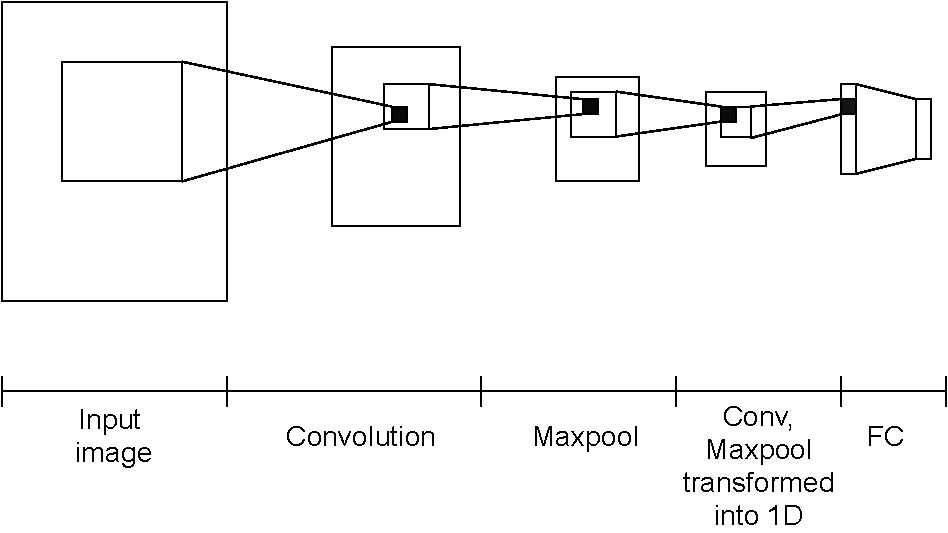
\includegraphics[width=.8\linewidth]{images/cnn.pdf}
        \caption{Example of CNN architecture}
        \label{fig:cnn}
    \end{figure}

\section{N-grams}
    N-grams is a method that is mostly used for word prediction
    \citep{speech2009Jurafsky:2009:SLP:1214993}. Given a sentence,
    \begin{center}
        \texttt{Please do not sit ...}
    \end{center}
    word \textit{on} or \textit{at} is more likely to follow instead
    of \textit{run} or \textit{bacteria}. In short, the previous task
    can be written as $P(w\vert h)$, probability of the next word $w$
    given some history part of sentence $h$. In previous case, the
    history $h$ is "\textit{Please do not sit}" and the probability in
    question is the following word $w$ will be "\textit{on}". To solve
    this task, counting the appearance of history $h$ followed by word
    $w$ can be used to retrieve the probability
    \citep{speech2009Jurafsky:2009:SLP:1214993}. Mathematically it can
    be written as follow,
    \begin{equation*}
        \label{eq:countingprob}
        P(\text{on} \vert \text{Please do not sit}) = 
        \frac{C(\text{Please do not sit on})}{C(\text{Please do not sit})}
    \end{equation*}
    Previous method can give good estimation, but because language is
    creative and new sentences generated every time, everything that
    exists on the internet is not enough to produce good estimate
    \citep{speech2009Jurafsky:2009:SLP:1214993}. On top of that, if
    the joint probability of the sequence would be calculated, there
    will be many estimations where each estimation is not exact
    because there is no way for the probability to be calculated given
    long sequence of preceding words because as stated above,
    language is creative
    \citep{speech2009Jurafsky:2009:SLP:1214993}. Given sequence of
    words $(w_1, w_2, \dots, w_n)$, the joint probability of these
    sequence can be calculated by using chain rule as follows,
    \begin{align}
        \label{eq:jointprob1}
        P(w_1, w_2, \dots, w_n) &= P(w_1)P(w_2 \vert w_1)P(w_3 \vert w_1, w_2) \dots
        P(w_n \vert w_1, w_2, \dots, w_{n-1}) \\
        \label{eq:jointprob2}
        &= \prod_{i=1}^n P(w_i \vert w_1, \dots, w_{i-1})
    \end{align}
    As shown on equation \ref{eq:jointprob1}, each occurrence of
    preceding sequence that followed by the desired word is estimated
    by counting the occurrence as shown in equation
    \ref{eq:countingprob} for the whole history.
    
    Instead of previous calculation, better way to calculate the word
    $W$ given history $h$ is needed because as stated above, language
    is creative making calculating exact probability impossible and
    there will be too many estimation if there is long sequence that
    precedes the target word. Hence n-grams has been introduced to
    approximate the probability of word $w$ from last few sequence of
    the history $h$ instead of a whole
    \citep{speech2009Jurafsky:2009:SLP:1214993}. For instance, only
    two preceding sequences will be taken into calculation.
    In other words, instead of following probability calculation,
    \begin{equation}
        P(\text{on} \vert \text{Please do not sit})
    \end{equation}
    the approximation of the probability will be as follows,
    \begin{equation}
        P(\text{on} \vert \text{not sit})
    \end{equation}
    In other words, the conditional probability then approximated by
    following equation,
    \begin{equation}
        \label{eq:condprobapprox}
        P(w_n \vert w_1, w_2, \dots, w_{n-1}) \approx P(w_n \vert w_{n-2}, w_{n-1})
    \end{equation}
    This approximation method then can be used for joint probability
    approximation as follows,
    \begin{equation}
        P(w_1, w_2, \dots, w_n) = \prod_{i=1}^n P(w_i \vert w_{i-2}, w_{i-1})
    \end{equation}
    for $P(w_j) = 1$ if $j < 1$.

    There are multiple n-grams model that are differentiated by the number
    of sequence used to estimate probability of the next word $w$. For
    example, preceding word in the history $h$ is used for estimating
    the next word $w$ in bigram model and two preceding words in the
    history $h$ is used in trigram model. In general, the window used
    for n-grams is configurable to the needs of the expected results.
    
    Another application of n-grams is that the sequence of character
    is used instead of sequence of words to estimate the probability.
    Differently from word n-grams, character n-grams are able to infer
    the morphological features of a written sentence or words
    \citep{kulmizev-etal-2017-power}. Instead of using history of
    words, character n-grams used history of character to predict the
    next character. All the equation is similar to the word n-grams. On
    top of that, character n-grams are really good for detecting
    patterns in case of typographical error and represented less
    sparsely compared to word n-grams since there are only so much
    character compared to the words made up from existing characters
    \citep{kulmizev-etal-2017-power}.
\chapter{Method}
\label{chap:method}

% This is the introduction to the thesis.\footnote{And this is a
% footnote.}  The conclusion is in Chapter on page
\section{Out-of-Vocabulary Model}
    \subsection{Sequence Feature Extraction}
        OOV problem was handled from quasi-generative perspective as
        aforementioned in chapter \nameref{chap:intro} by using neural
        language model under assumption that there is a form that
        could generate embedding for the original embedding. Hence
        that, the original vocabulary and its embedding were used for
        training the model to generate the embedding. In chapter
        \nameref{chap:intro}, reasons why \textsc{Mimick} could
        perform worse is because the OOV embedding is generated from
        the last hidden states of the bi-LSTM and the hidden states is
        controlled by cell gates $C_t$ making the information that is
        carried on is the most recent information. If at certain time
        step $t$ the cell gates decided to forget past information,
        then the early information might not be coded into the hidden
        state. On top of that, there are evidences that recurrent
        architecture could perform worse than CNN for sequence
        modelling \citep{empirical2018shaujie}. 
        
        If explained formally, when $C_t = 0$ from equation
        \ref{eq:lstm:C_t}, hidden state from equation
        \ref{eq:lstm:h_t} will also be $0$, resetting to its starting
        state, rendering hidden states prior to time $t$ gone. This
        problem can be solved by using bi-LSTM, since bi-LSTM processes
        sequence in forward and reverse order making both early and
        later sequences held by the last hidden state for each reverse
        LSTM and forward LSTM respectively. Another problem might
        arise when we need to divide sequence into more than three
        subsequence as shown on figure \ref{fig:subsequence}. Hence
        another approach is needed since intermediate subsequence
        might get deleted or carried along with the later sequences
        even with bi-LSTM. Another method that might be able to solve
        this problem for \textsc{Mimick} is by increasing hidden size
        and hope that it will be able to compensate the sequence that
        is dropped by the cell gate in the other hidden cell.
        \begin{figure}
            \begin{align*}
                &un \vert recogniz \vert able \\
                &inter \vert national \vert ities \\
                &oto \vert rhino \vert laryngolog \vert ical \\
                &hepatico \vert chol \vert angio \vert gastro \vert stomy
            \end{align*}
            \caption{Word examples with three or more subsequences}
            \label{fig:subsequence}
        \end{figure}

        \begin{figure}
            \begin{align*}
                unrecognizable : &unre \vert nrec \vert reco \vert ecog \vert cogn \vert ogni \vert gniz \vert niza \vert izab \vert\\ 
                &zabl \vert able\\
                internationalities : &inte \vert nter \vert tern \vert erna \vert rnat \vert nati \vert atio \vert tion \vert iona \vert\\
                &onal \vert nali \vert alit \vert liti \vert itie \vert ties\\
                otorhinolaryngological : &otor \vert torh \vert orhi \vert rhin \vert hino \vert inol \vert nola \vert olar \vert lary \vert \\
                &aryn \vert ryng \vert yngo \vert ngol \vert golo \vert olog \vert logi \vert ogic \vert gica \vert\\
                &ical\\
                hepaticocholangiogastrostomy : &hepa \vert epat \vert pati \vert atic \vert tico \vert icoc \vert coch \vert ocho \vert chol \vert hola \vert\\
                & olan \vert lang \vert angi \vert ngio \vert giog \vert ioga \vert ogas \vert gast \vert astr \vert stro \vert\\
                &tros \vert rost \vert osto \vert stom \vert tomy
            \end{align*}
            \caption{4-grams examples}
            \label{fig:4grams}
        \end{figure}

        For all subsequence to be processed, a method that accounts
        for the whole sequence yet still able to divides the whole
        sequence into subsequences is needed. Consequently, n-grams
        was chosen because this method splits word into sequence of
        characters depending on the chosen window size as shown on
        figure \ref{fig:4grams}. Before processing the n-grams, the
        word first split into sequence of characters and then each
        character is transformed into embedding and processed with CNN
        inspired from CNN word n-grams \citep{convolutional2014kim}.
        Those sequences of character embeddings then fed into learning
        algorithm. This idea is similar to how human tries to
        recognize an unseen word by reading subword that is
        understandable beforehand when no explanation or context were
        given. In other words, given sets of vocabulary $\mathcal{V}$
        with size $\vert\mathcal{V}\vert$ and pretrained embeddings
        $\mathcal{W}^{\vert\mathcal{V}\vert \times d}$ for each word
        $w_{i} \in \mathcal{V}$ that is represented as a vector $e_i$
        with $d$ dimension, the model is trained to map function
        $f:\mathcal{V} \rightarrow \mathbb{R}^d$ that minimizes the
        loss function,
        \begin{equation}
            \label{eq:lossfn}
            \mathcal{L} = \Vert f(w_i) - e_i \Vert^{2}_2
        \end{equation}
        This approach is similar to \textsc{Mimick}
        \cite{mimicking2017Pinter} approach. The text input was
        represented as a sequence of character $[c_1, c_2, \dots,
        c_m]$ for $c_i \in \mathcal{C}$. Those sequence then
        transformed as sequence of vectors $g_i$ with $b$ dimension by
        using character embeddings $\mathcal{G}^{\vert \mathcal{C}
        \vert \times b}$. For simplicity, sequence of $[g_1, g_2,
        \dots, g_m]$ will be called $\{g\}^m$. $\{g\}^m$ becomes
        2-dimensional matrix that has size of $m \times b$. In
        summary, given word $w$ was transformed using embedding
        generation function $h$ into $\{g\}^m$ as shown on equation
        \ref{eq:word2charemb}.

        \begin{equation}
            \label{eq:word2charemb}
            h: w \rightarrow \{g\}_1^m
        \end{equation}

        To process $\{g\}^m$ like an n-grams, CNN is used inspired
        by CNN n-grams implementation by \cite{convolutional2014kim}.
        CNN n-grams is basically a method to do convolution on matrix
        by using a kernel $k_i^{b \times n} \in K$ for $n$ is the
        window size of the grams and $b$ is the dimension size of the
        character embedding. This operation is represented with $*$
        symbol as stated in equation \ref{eq:conv_d:2}. This operation
        produced another vector $\hat{l}$ that represents the value of
        each grams, then non-linearity was applied to this vector by
        using ReLU activation,
        \begin{equation}
            \label{eq:relu}
            ReLU(x) = max(0,x)
        \end{equation}

        Several kernel was used to learn several features for
        producing embeddings. Each of these kernel was responsible to
        find grams that were affecting the results, thus the vector
        $\hat{l_i}$ that is results of convolution $\{g\}^m * k_i$
        will be maxpooled to produce one number. In details, from
        given sequence of character embedding $\{g\}^m$, only gram
        that produces the highest value when convoluted by using
        kernel $k_i$ will be processed. Since, there are $\vert K
        \vert$ number of filter, $\vert K \vert$ number of grams will
        be considered to be important to the results. Furthermore, by
        using several window sizes for n-grams (bigram, trigram, etc.)
        by changing the size of the kernel more features will be able
        to be learned. For instance bigram will has a kernel with size
        $b \times 2$, trigram will has a kernel with size $b \times
        3$, and so on and so forth, making the different sizes of
        n-grams can be trained together only then concatenated later.

    \subsection{Embedding Generation}
        After the features were able to be extracted, those features
        then concatenated and fed into fully connected layer with
        output size matching the pretrained embedding $\mathcal{W}$
        dimension $d$ with non-linear activation function $Hardtanh$
        matching the maximum and minimum bound of the pretrained
        embedding $\mathcal{W}$ resulting a new embedding vector
        $\tilde{e}$. The fully connected layer consists of one hidden
        layer and one output layer with batch normalization before
        each layer to further sped up the training convergence
        according to \cite{batchnorm:DBLP:journals/corr/IoffeS15}.
        This normalization layer basically maintains that the
        distribution of each minibatch remains similar so that
        covariance shift is minimized in the training process
        \citep{batchnorm:DBLP:journals/corr/IoffeS15}. This process
        was done by applying transformation on each minibatch to a
        certain mean and variance
        \citep{batchnorm:DBLP:journals/corr/IoffeS15}. This mean and
        variance are learnable parameters. Let minibatch $\mathcal{B}
        = {x_1, x_2, \dots, x_m}$, following operations were applied,
        \begin{align}
            \label{eq:bn:mu}
            \mu_{\mathcal{B}} &= \frac{1}{m} \sum_{i=1}^m x_i\\
            \label{eq:bn:var}
            \sigma^2_{\mathcal{B}} &= \frac{1}{m} \sum_{i=1}^m \left(x_i - \mu_{\mathcal{B}}^2\right)\\
            \label{eq:bn:norm}            
            \tilde{x}_i &= \frac{x_i - \mu_{\mathcal{B}}}{\sqrt{\sigma^2_{\mathcal{B}} + \epsilon}}\\
            \label{eq:bn:transform}            
            BN(x_i) &= \gamma\tilde{x_i} + \beta
        \end{align}
        Equation \ref{eq:bn:mu} and equation \ref{eq:bn:var} tries to
        find the mean and variance to normalize the minibatch by
        equation \ref{eq:bn:norm}. After all of the data in the
        minibatch $\mathcal{B}$ were normalized, the data then scaled
        by parameter $\gamma$ and shifted by parameter $\beta$ as
        shown in equation \ref{eq:bn:transform}. By making the
        parameters $\gamma$ and $\beta$ learnable, the model will
        adjust this process in the training process.

        After all the process above was done, the generated embedding
        vector $\tilde{e}$ was produced.
        % then passed into a highway network to
        % decide whether some information should be carried or should be
        % forgotten to obtain a new sets of embedding. Given the output
        % of max-over-time pooling $m$, The highway network is
        % calculated by the following equation, 
        % \begin{align}
        %     \label{eq:highway}
        %     t &= ReLU(f(\mathbf{W}m + b))\\
        %     \mathbf{Z} &= t \odot g(\mathbf{W_{\mathbf{H}}}m + b_{\mathbf{H}}) + (1-t) \odot m
        % \end{align}
        The complete process from input word, feature extraction,
        until predicting embedding is shown on figure \ref{fig:model}.
        \begin{figure}
            \centering
            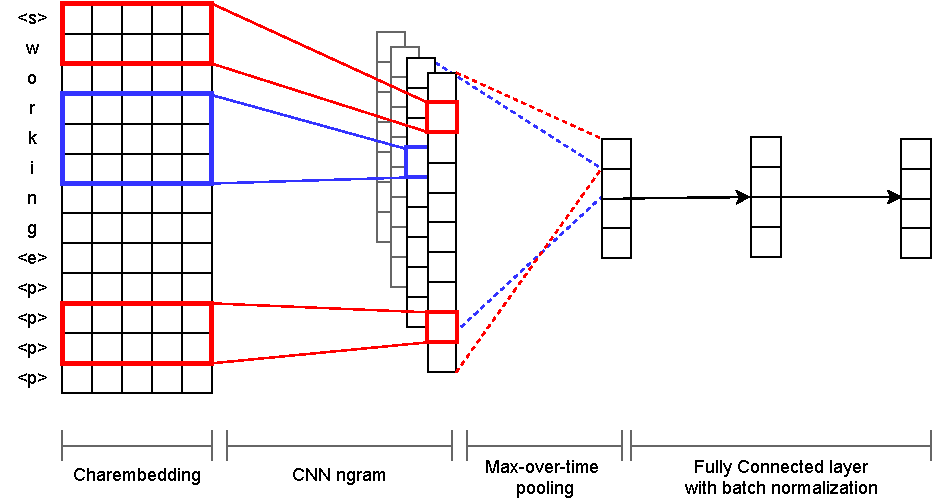
\includegraphics[width=.8\linewidth]{images/model_batchnorm.pdf}
            \caption{OOV Inferencing Model}
            \label{fig:model}
        \end{figure}
        On figure \ref{fig:model}, starting and ending token were
        added at the beginning and the end of the word respectively.
        Furthermore, padding token was added if the input word was
        shorter than the longest input size in the minibatch. The
        padding token is a zero vector $\vec{0}$ and $\vec{0} * k =
        \vec{0}$ for any $k$. This is to ensure that part of input
        that got padded does not goes through maxpool layer since only
        grams that has highest value can goes through the next layer
        and minimum value of ReLU is 0 thus the result of maxpooling
        it will be 0. The reason for this is so that various length of
        words are able to be processed by the model.

    \subsection{Error and Backpropagation}
        The predicted embedding $\tilde{e}$ from the model then
        compared with the original embedding $e$ to adjust all of the
        parameters for the neural network using mean squared error
        function,
        \begin{equation}
            \label{eq:errorf}
            Error = \frac{1}{2} \Vert e - \tilde{e} \Vert ^{2}_2
        \end{equation}
        By minimizing $Error$, it is similar to minimizing
        $\mathcal{L}$ shown in equation \ref{eq:lossfn}. The error
        then backpropagated to fine-tune the neural network
        parameters, character embedding $\mathcal{G}$, the kernel $k
        \in K$, and the batch normalization parameters $\gamma$ and
        $\beta$.
        
\section{Measuring Performance on Downstream Tasks}
    In natural language modeling (NLP), there are several tasks that
    make use of word embedding. Hence that, the generated embeddings
    from the model can be evaluated by using those downstream tasks.
    The results then compared with the state-of-the-art OOV handling
    model \textsc{Mimick} \citep{mimicking2017Pinter}.
    
    \subsection{Part-of-Speech Tagging}
        Part-of-speech tagging or POS-tagging is a task of classifying
        usage of words in sentence or corpus based on the grammatical
        usage of the word \citep{robustpostag2018horsmann}, for
        example: verb, noun, adverb, etc. Given sentence $S = \{w \in
        \mathcal{V} \vert ((w_1, t_1), (w_2, t_2), \dots, (w_n,
        t_n)\}$ with its POS-tag $t_i$, each word $w_i$ that exist in
        the vocabulary $w_i \in \mathcal{V}$ and $w_i \in S$ was
        transformed into embedding $e_i$. For the OOV, every sequence
        of the characters building a word transformed into sequence of
        character embedding $\{g\}_{i}^m$ using model represented in
        equation \ref{eq:word2charemb} then the embedding
        $\tilde{e}_i$ was predicted using the OOV handling model, else
        the original embedding was used if the word exist inside the
        vocabulary $\mathcal{V}$. This was done by masking the output
        of the OOV handling model and the original embedding in the
        following way,
        \begin{align}
            \label{eq:embeddingmask}
            embedding &= mask \odot e_i + (1-mask) \odot \tilde{e}_i\\
            mask &=
            \begin{cases}
                \vec{1} & \text{if }\ w_i \in \mathcal{V}\\
                \vec{0} & \text{otherwise}
            \end{cases}
        \end{align}        
        This way the gradient would not flow into the OOV model if the
        word exist in $\mathcal{V}$ and will flow if the word does not
        exist in $\mathcal{V}$ and the embedding was generated by the
        OOV model.

        The sequence of embeddings $\tilde{e}_i$ or $e_i$ then fed
        into bi-LSTM and the output was passed through LogSoftmax
        activation function,
        \begin{equation}
            \label{eq:logsoftmax}
            LogSoftmax(x_i) = log \Bigg(\frac{exp(x_i)}{\sum_j exp(x_j)}\Bigg)
        \end{equation}
        to classify the POS-tag $t$. To ease up computation time,
        adaptive LogSoftmax is used \citep{grave2018efficientsoftmax}.
        Instead of calculating the whole tag classification, the
        frequent and infrequent classes were separated thus there were
        many chances that only frequent classes needed to be calculated
        before trying to calculate the infrequent classes. After
        calculating the loss, stochastic gradient descent was used to
        optimize the parameters of the model. The complete process of
        POS-tagging process is shown in figure \ref{fig:postag}. After
        training was done, the accuracy of the POS-tagger based on
        different OOV handling model were compared.

        \begin{figure}
            \centering
            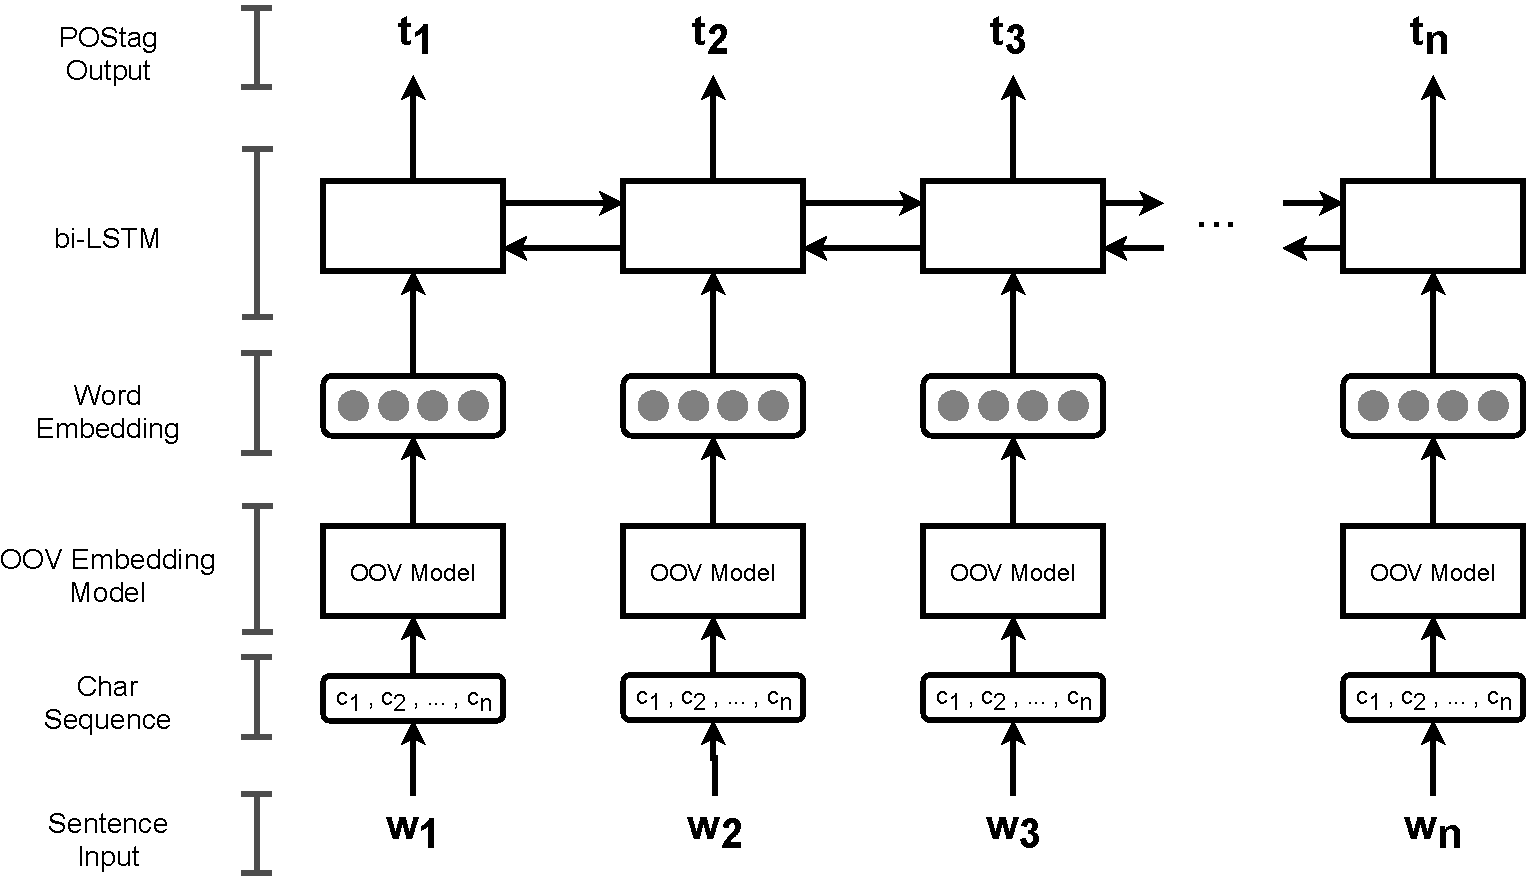
\includegraphics[width=.8\linewidth]{images/postag.pdf}
            \caption{Pos-tagging Process}
            \label{fig:postag}
        \end{figure}
 
    \subsection{Word Similarity Tasks}
        Word similarity tasks is basically task to evaluate the
        similarities between two words based on human given scores. In
        practice, several human subjects were given pairs of words and
        asked to score its similarities. Those scores then will be
        used to determine the agreements between subjects that certain
        word pairs have stronger connection and the others are weaker.
        In order to calculate the agreements between the OOV generated
        embedding and the data that is scored by human, Spearman's
        rank correlation coefficient is used. Firstly, given a pair
        $(w_1, w_2)$, the cosine distance of the embedding
        $\tilde{e}_1$ and $\tilde{e}_2$ based on the generated
        embedding from OOV model for $w_1$ and $w_2$ calculated
        respectively using the following equation,

        \begin{equation}
            \label{eq:cosinesim}
            CosineSimilarity(e_1, e_2) = \frac{e_1 \cdot e_2}{\Vert e_1 \Vert \Vert e_2 \Vert}
        \end{equation}

        After all of the cosine distance for all pairs were calculated,
        Spearman rank's correlation from the dataset and the generated
        embedding are calculated by using equation \ref{eq:spearman}
        and by using equation \ref{eq:spearmantied} when no tied ranks
        exists. The results of both \textsc{Mimick} and the proposed
        model from several word similarity datasets then averaged and
        compared.
        
        \begin{align}
            \label{eq:spearman}
            \rho    &= \ddfrac{n\sum_{i=1}^n u_i v_i - \Bigg( \sum_{i=1}^n u_i \Bigg) \Bigg( \sum_{i=1}^n v_i \Bigg)}{\sqrt{\Bigg[ n \sum_{i=1}^n u_i^2 - \Bigg( \sum_{i=1}^n u_i \Bigg)^2 \Bigg] \Bigg[ n \sum_{i=1}^n v_i^2 - \Bigg( \sum_{i=1}^n v_i \Bigg)^2 \Bigg] }}\\
            \label{eq:spearmantied}            
                    &= 1 - \ddfrac{6 \sum_{i=1}^n d_i^2}{n(n^2 - 1)}\ \text{where}\ d_i = u_i - v_i
        \end{align}

\chapter{Implementation}
\label{chap:implementation}

\section{Preparation}
    \subsection{Dataset Preparation}
        \subsubsection{Character Embedding}
            The character dictionary consists of first 128 ASCII
            characters with deletion for non character types (the
            first 32 ASCII symbols). Then the character embedding was
            initialized by randomly generated from normal distribution
            with $\mu = 0$ and $\sigma = 1$. Another entries such as
            unknown token \textit{\textless unk\textgreater}, starting
            token \textit{\textless s\textgreater}, ending token
            \textit{\textless e\textgreater} and padding token
            \textit{\textless p\textgreater} were added along with the
            random character embedding initialization.

        \subsubsection{Pre-trained Word Embedding}
            In order to train the model, pre-trained embedding was
            needed since the model will tries to predict embedding
            from known vocabulary $v \in \mathcal{V}$ with its known
            embedding $e \in \mathcal{W}$. For this purpose, word2vec
            which trained on Google news dataset using skip-gram model
            containing 3 million words and phrases (name, hyperlink,
            connected words, etc.) was used
            \citep{Distributed2013mikolov}. The embedding contains
            300-dimensional vectors. Word2vec \footnote{Pretrained
            embedding available at 
            \url{https://code.google.com/archive/p/word2vec/}}
            contains words that frequently appears as a phrase, for
            instance the word New and Jersey appears frequently side
            by side because both of this words form name of a state in
            United States of America. In the original vocabulary, this
            phrase might be written as "New\_Jersey", thus for the
            purpose of simplifying the input and the downstream tasks
            those phrases was not included. On top of phrases, the
            original vocabulary also includes hyperlinks which usually
            contains "http". Such entries will also be removed. Only
            first 40 thousands words with removal if the word contains
            "\_" (underscore) or "http" is used in this research.
            
            Another pre-trained embedding is
            polyglot\footnote{Pretrained embedding available at
            \url{https://polyglot.readthedocs.io/en/latest/index.html}}
             which contains multilingual embeddings
            \citep{polyglot2013alrfou}. For this research, only
            English embedding that contains around 100.000 words with
            60-dimensional vector representations will be used. This
            pre-trained embedding was also used in OOV handling model
            \textsc{Mimick} which used as baseline model
            \citep{mimicking2017Pinter}.

            Dict2vec\footnote{Pretrained embedding available at
            \url{https://github.com/tca19/dict2vec}} is yet another word
            embedding that trained based on the definition of a word in
            dictionary \citep{dict2vect2017tissier}. Each words
            location in Euclidean space was determined by the
            appearance of another words in the definition that is
            defined by the Cambridge dictionary. Originally, this
            embedding was tested using word similarity tasks with
            removal of OOV words.

        \subsubsection{Word Similarity Dataset}
            Several word similarity datasets were used in order to
            increase the pair examples since for the datasets that are
            collected, the highest number of pairs is just above 3000
            pairs. Those datasets used for word similarity tasks are
            Card-660 \citep{card660:pilehvar-etal:2018}, MC-30
            \citep{mc30:strongContextualHypothesis}, MEN-TR-3k
            \citep{mentr3k:bruni-etal-2012-distributional}, MTurk-287
            \citep{mturk287:Radinsky:2011:WTC:1963405.1963455},
            Mturk-771
            \citep{mturk771:Halawi:2012:LLW:2339530.2339751}, RG-65
            \citep{rg65:Rubenstein:1965:CCS:365628.365657},
            RW-STANFORD \citep{rw:luong-etal-2013-better}, SimLex-999
            \citep{simlex999:hill2014}, YP130
            \citep{yp130:inproceedings}, VERB143
            \citep{vp143:baker-etal-2014-unsupervised}, and Wordsim353
            \citep{wordsim353:2002:PSC:503104.503110}.

    \subsection{Programming Language and Tools}
        The model was trained using PyTorch 1.1.0 machine learning
        library on top of Python 3.6 \citep{pytorch2017paszke}. Most
        of the basic functions, for instance 2d convolution layer, 2d
        maxpool layer, fully connected layer, bi-LSTM, and many
        activation functions and loss functions, and other mathematical
        functions were already implemented as a library in PyTorch,
        thus will serve enough for the purpose of this research.
            
    \subsection{Hardware}
        The model was trained on the freely available Google
        Colaboratory\footnote{Google Colaboratory available at
        \url{https://colab.research.google.com/}} which gives
        randomized hardware specification based on the availability,
        thus the exact hardware configuration used cannot be
        determined. The GPU engine was used to train the model.
        Nevertheless, this only affects the time needed to train the
        model and not the results.

\section{Training}
    \subsection{Training OOV model}
        Firstly, the pretrained embeddings acted as the datasets were
        shuffled and split up into train-val set with $80\%$ and
        $20\%$ quota respectively with minibatch size of 64. The word
        $w_i \in \mathcal{V}$ becomes the input of the model and the
        word embedding $e_i \in \mathcal{W}$ becomes the target. The
        input word split into sequence of characters and starting
        token \textit{\textless s\textgreater} and ending token
        \textit{\textless e\textgreater} were added at the beginning
        and at the end of the word respectively. For every minibatch,
        the longest word will be used as the maximum length. Every
        word that was shorter than the longest word will be padded
        with a padding token \textit{\textless p\textgreater}.
        % For the proposed model, padding token was added at the
        % beginning and at the end of the word to make single
        % character entries at the beginning and at the end of the
        % word to be able to be processed by the CNN. 
        The sequence of characters then transformed into character
        embeddings then processed by the model producing the predicted
        word embedding. The \textsc{Mimick} model was trained with
        learning rate $lr = 0.01$ for polyglot and $lr = 0.1$ for the
        rest with no dropout as dropout does not work well just as in
        the original implementation of \textsc{Mimick}
        \citep{mimicking2017Pinter}. On the other hand, CNN model was
        performing better with dropout when the model was pre-tested
        using different parameters. In summary, the hyperparameters
        setting is shown in table \ref{tab:hyperparameter}.

        \begin{table}[]
            \centering
            \caption{OOV Handling Model Parameters}
            \label{tab:hyperparameter}
            \begin{tabular}{@{}lcc@{}}
                \toprule
                \textbf{Hyperparameter} & \multicolumn{1}{c}{\textbf{\textsc{Mimick}}} & \multicolumn{1}{c}{\textbf{CNN}} \\ \midrule
                Train-Val split & \multicolumn{2}{c}{$80\%$; $20\%$}\\
                Batch size & \multicolumn{2}{c}{64} \\
                Epoch & \multicolumn{2}{c}{100} \\
                Momentum & \multicolumn{2}{c}{0.5} \\
                Learning Rate ($\eta$) & [0.01; 0.1] & 0.1 \\
                Dropout & 0 & 0.5 \\
                Num features & [50; 100; 200; 300] & [20; 50; 100; 150] \\ \bottomrule
            \end{tabular}
        \end{table}

        For the proposed model, the character embeddings were
        processed with CNN n-grams following
        \cite{convolutional2014kim} architecture for word n-grams.
        N-grams with window size $n = [2, 3, 4, 5, 6, 7]$ were used
        with respective kernel size $n \times b$ to simulate n-grams.
        Different sets of n-grams sizes, for instance $n = [2, 3, 4]$
        or $n = [5, 6, 7]$ can be used instead of the whole n-grams
        sizes. The results on the downstream tasks for the different
        settings then compared with the whole model and with the
        \textsc{Mimick} model.
        
        After max-over-time pooled, the vector representation then
        passed into two layers of fully connected network with batch
        normalization layer for each layer to produce the predicted
        word embedding. Batch normalization helps with the training
        process by making all of the minibatch data to have similar
        distribution for each layer
        \citep{batchnorm:DBLP:journals/corr/IoffeS15}. The error then
        calculated using Mean Squared Error as mentioned on equation
        \ref{eq:errorf} then back-propagated to update the weights.

        Similar datasets were used to train \textsc{Mimick} with
        parameters taken from the original paper
        \citep{mimicking2017Pinter}. To find the optimal parameters
        such as learning rate, number of features/hidden neurons, and
        number of epoch, several number of tests with different number
        of parameters needed to be done as preliminaries. The summary
        of the hyperparameters are after the preliminary tests are
        shown in table \ref{tab:hyperparameter}.

        % \begin{table}[]
        %     \centering
        %     \caption{OOV Handling Model Parameters}

        %     \begin{tabular}{@{}lcl@{}}
        %         \toprule
        %         \textbf{Hyperparameter} & \multicolumn{1}{l}{\textbf{\textsc{Mimick}}} & \textbf{CNN} \\ \midrule
        %         Learning Rate ($\eta$) & \multicolumn{2}{c}{0.1} \\
        %         Batch size & \multicolumn{2}{c}{64} \\
        %         Epoch (word2vec) & \multicolumn{2}{c}{1000} \\
        %         Epoch (polyglot-en) & \multicolumn{2}{c}{100} \\
        %         Epoch (dict2vec) & \multicolumn{2}{c}{1000} \\
        %         Momentum & \multicolumn{2}{c}{0.5} \\
        %         Num features & [100; 700] & \multicolumn{1}{c}{100} \\ \bottomrule
        %     \end{tabular}
        % \end{table}
    
\section{Evaluating with Downstream Tasks}
    \subsection{Part-of-Speech Tagging}
        For POS-tagging task, the readily brown corpus and its tagset
        from NLTK\footnote{Available at \url{https://www.nltk.org/}}
        were used to test the performance of the model as well as the
        previous \textit{state-of-the-art}. In this task, two kinds
        of evaluation methods were done. Before going into the method,
        there are several steps to prepare the datasets for training
        the POS-tagger. Firstly, the POS-tag dataset words were
        collected as sets $\mathcal{S}$. This was done in order to
        collect the vocabulary uniquely since in Python set elements
        are unique. Secondly, each elements in the set $\mathcal{S}$
        was scanned whether it is in-vocabulary or out-of-vocabulary.
        If the element turns out to be OOV, this element which is a
        word, will be added into the vocabulary $\mathcal{V}$ and its
        embedding, either a zero vector, a randomly initiated value,
        or a generated embedding from the OOV model depending by the
        method used, will be added to the original embedding
        $\mathcal{W}$. The dataset were split up into 80\% for train
        set and 20\%  for test set.
        
        The first method was to train the POS-tagger by using a
        pre-trained embedding. The original pre-trained embedding entries
        $\mathcal{W}$ were concatenated with the OOV model predicted
        embeddings $f(\text{OOV})$ so that each word $v \in
        \mathcal{V}$ has vector representation. In short, the new
        embedding $\mathcal{W}_{new} = \mathcal{W} \cup
        f(\text{OOV})$. The new pre-trained embedding
        $\mathcal{W}_{new}$ will not be trained in this method by
        setting the parameters to be fixed values.
        
        The second method was to train the OOV model together with the
        POS-tagger. For this method, for each OOV entries added into
        the vocabulary $\mathcal{V}$, a zero vector representing the
        embedding of the OOV will be added to the embedding
        $\mathcal{W}_{new}$ that later on replaced with the
        generated embedding $f(\text{OOV})$ if the input word is OOV
        as explained in the equation \ref{eq:embeddingmask} by masking
        the entries. Thus the OOV model will still be trained if the
        input turns out to be OOV while it is non-trainable if it is
        in-vocabulary input. Both of the models were used here then
        the accuracies were compared.

        Lastly, it is similar to the second method but the pre-trained
        embedding was set to be a trainable parameters. Using similar
        method of masking, the gradient will flow separately depending
        on the embedding used, whether it is from the pre-trained
        embedding or from the embedding generated by the OOV model.

        On top of different method used in this task, the sentence
        length was limited to 5 words. If the sentence length is less
        than 5 words then padding tokens were added at the end of the
        sentence to make the length becomes 5 words and if the
        sentence's length is more than 5 words, the slice of the
        sentence were randomly selected. Note that this padding token
        is different than the padding token of the character
        embedding. The padding token \textit{\textless p\textgreater}
        is a zero vector with dimension similar with the pre-trained
        embedding $\mathcal{W}$. The POS-tagger were trained with 100
        epoch with 6 different seeds for the random number generation.
        The learning rate used was $0.1$ with dropout for CNN model
        $0.5$ and no dropout for \textsc{Mimick} since it makes the
        model performs worse based on preliminary tests. The momentum
        used for the training was $0.5$. In summary the parameters
        used are shown in table \ref{tab:hyperparameterpostag}.

        \begin{table}[]
            \centering
            \caption{POS-Tagger Model Parameters}
            \label{tab:hyperparameterpostag}
            \begin{tabular}{@{}lcc@{}}
                \toprule
                \textbf{Hyperparameter} & \multicolumn{1}{c}{\textbf{\textsc{Mimick}}} & \multicolumn{1}{c}{\textbf{CNN}} \\ \midrule
                Learning Rate ($\eta$) & \multicolumn{2}{c}{0.1} \\
                Batch size & \multicolumn{2}{c}{64} \\
                Epoch & \multicolumn{2}{c}{100} \\
                Momentum & \multicolumn{2}{c}{0.5} \\
                Training seed & \multicolumn{2}{c}{[64; 20; 128; 0; 5;
                10]} \\
                Dropout & 0 & 0.5 \\ 
                \bottomrule
            \end{tabular}
        \end{table}

    \subsection{Word Similarity}
        Word similarity task is quite straight forward. Given pairs of
        words, if the word is an OOV in the pre-trained embedding, the
        word embeddings were predicted from OOV models then the cosine
        similarity of the word embeddings were calculated and compared
        between two models, else the original embedding from the
        pre-trained embedding was used. 
        
        The baseline embeddings used for this task, dict2vec
        \citep{dict2vect2017tissier}, was also tested using random OOV
        embedding by randomly giving OOV word random embedding and
        choosing the maximum results from five tries. On top of that,
        other two pre-trained embedding used in this research were
        also used for comparing results. The results were then
        compared between two models.
\chapter{Results and Discussion}
\label{chap:results}
    \section{OOV handling model}
        After training the model was done, some OOV words were fed
        into the model and 5 nearest in-vocabulary words were
        calculated for sanity check and it is shown on the table
        below. Some of the input that is used were similar to the one used in testing
        \textsc{Mimick} on the original paper for Polyglot embedding
        for English. Both model CNN and \textsc{Mimick} results
        for nearest neighbor that were trained with Polyglot are shown
        in Table \ref{tab:nearest:cnn-polyglot} and Table
        \ref{tab:nearest:lstm-polyglot} respectively. The number of
        features for \textsc{Mimick} and CNN was 100.

        The first word was "hurtling", typographical error from the
        word hurting. For this word, both model seemed to be able to
        locate that the nearest neighbor was another verb with suffix
        \textit{-ing}. Interestingly for CNN, it could relate this
        word with action that might induce pain thus hurting a
        subject. The second word was "expectedly". Both model were
        able to predict that the nearest neighbor was another word
        with suffix \textit{-ly}. The third input word was "Actively".
        For this input, \textsc{Mimick} predicted that this word was a
        name which the first character in the word is capitalize, thus
        the nearest neighbor was a name. On the other hand, CNN
        predicted that this was some word with suffix \textit{-ly} and
        the first character was capitalized. The next word was
        "corduroy", which is a pattern in textile. CNN model were able
        to predict that one of the nearest neighbor was "garment". The
        next input was "question-and-answer". This input was constructed
        from 3 words connected with dash (-) symbol. CNN model
        predicted that the nearest neighbor were activities that the
        subjects do, for instance "hostess" and "recruiter". The last
        input was a number "1657". \textsc{Mimick} predicted that the
        nearest neighbor was mathematical function in latex for example
        "\textbackslash exp", while CNN predicted the nearest neighbor
        to be an abbreviation.

        From those results, both models were able to predict the
        nearest neighbor that might be related to each other for some
        cases, but this results were highly dependent on the pre-trained
        embedding that was used to train the OOV handling model. If both model
        were trained using Word2vec, then for input word "hurtling"
        and "corssing" produced nearest neighbor "turning", "putting",
        "squeezing", "pushing", "talking", and "pulling" in different
        order for both model.
        
        % The first test word were an abbreviation "MCT" with length of
        % three characters and all-capitalize. Both model were able to
        % predict that the nearest neighbors are also another
        % abbreviation. For name as input, "McNeally" and "Vercelloti",
        % both model were able to predict the nearest neighbor to be
        % name as well, as shown on Table \ref{tab:nearest:cnn-word2vec}
        % and Table \ref{tab:nearest:lstm-word2vec}. For "McNeally" the
        % nearest neighbor were English name for male for both models.
        % Interestingly for "Vercellotti", \textsc{Mimick} predicted
        % that the nearest neighbor was former American baseball player,
        % while CNN predicted that the nearest neighbor was Ukrainian
        % politician. For an adjective input "Secretive", both model
        % were predicted that the nearest neighbors are group of verbs,
        % nouns, adjectives, and adverbs. Both models were also able to
        % handle typography error like "corssing" and "developiong",
        % only that CNN model nearest word were "developing" while
        % \textsc{Mimick} were a verb that has suffix \textit{-ing}. The
        % nearest neighbors for corssing were also verb with suffix
        % \textit{-ing}. Interestingly, for both model, nearest neighbor
        % for flatfish has no correlation at all.

        % Similar nearest neighbors were also produced by the model when
        % trained with polyglot \citep{polyglot2013alrfou} only with
        % different set of words for each input.

        \begin{table}[H]
          \begin{center}
            \caption{Nearest Neighbors Mimick (Polyglot)}
            ~\\
            \footnotesize
            \label{tab:nearest:lstm-polyglot}
            \begin{tabular}{l|l}
              \textbf{OOV Word} & \textbf{Nearest Neighbors}\\
              \hline
              hurtling & inflating compromising concealing grasping channeling\\
              expectedly & materially substantively sensibly energetically ethically\\
              Actively & Harrold Wasson Wheatcroft Dever Covey\\
              corduroy & heartbeat kink delicacy diaper damper\\
              question-and-answer & barometer bottleneck ventilator slowdown spurt\\
              1657 & \textbackslash exp \textbackslash frac\{n \textbackslash frac\{\# sqrt x\^{}\{\\
            \end{tabular}
          \end{center}
        \end{table}

        \begin{table}[H]
          \begin{center}
            \caption{Nearest Neighbors CNN (Polyglot)}
            ~\\
            \footnotesize
            \label{tab:nearest:cnn-polyglot}
            \begin{tabular}{l|l}
              \textbf{OOV Word} & \textbf{Nearest Neighbors}\\
              \hline
              hurtling & pulling whipping catching shaking burning\\
              expectedly & frequently legitimately painfully inappropriately purposefully\\
              Actively & Easily Potentially Entirely Merely Displaying\\
              corduroy & basket garment wedge medium nutrient\\
              question-and-answer & hostess dentist recruiter carer pastime\\
              1657 & GER BO INT SEP AGP\\
            \end{tabular}
          \end{center}
        \end{table}

        % \begin{table}[H]
        %   \begin{center}
        %     \caption{Nearest Neighbors Mimick (word2vec)}
        %     ~\\
        %     \footnotesize
        %     \label{tab:nearest:lstm-word2vec}
        %     \begin{tabular}{l|l}
        %       \textbf{Word} & \textbf{Nearest Neighbors}\\
        %       \hline
        %       MCT & AWS NIC BTC ATS AAR\\
        %       McNeally & Wagstaff Lanning O'Dell Kellman Wolk\\
        %       Vercellotti & Antonelli Cardinale Veron Villani Sabatini\\
        %       Secretive & Entrepreneurial Predictive Screening Routine Themed\\
        %       corssing & compromising balancing inflating pulling reversing\\
        %       flatfish & slimy fluffy supple flaky greasy\\
        %       compartmentalize & formalize scrutinize validate redefine formulate\\
        %       pesky & nutty sensuous dreamy pungent euphoric\\
        %       lawnmower & lifeguard laborer tradesman bathhouse boarder\\
        %       developiong & compromising channeling sacrificing cementing alienating\\
        %       hurtling & pounding pulling catching compromising whipping\\
        %       expectedly & painfully strangely admirably energetically legitimately\\
        %       prople & figure circle mask plot pattern\\
        %       nrews & counters messes tips dials timings\\
        %       newss & promise knack friendliness hype bounce\\
        %       googel & wand contraption handkerchief talisman noose\\
        %     \end{tabular}
        %   \end{center}
        % \end{table}
        
        % \begin{table}[H]
        %   \begin{center}
        %     \caption{Nearest Neighbors Mimick (Polyglot)}
        %     ~\\
        %     \footnotesize
        %     \label{tab:nearest:lstm-word2vec}
        %     % \setlength\extrarowheight{2pt}
        %     \begin{tabularx}{1.1\textwidth}{|c|L|c|L|}
        %       \hline
        %       \textbf{OOV} & \textbf{Nearest Neighbors} & \textbf{OOV} & \textbf{Nearest Neighbors}\\
        %       \hline
        %       MCT & AWS NIC BTC ATS AAR & McNeally & Wagstaff Lanning O'Dell Kellman Wolk\\ \hline
        %       Vercellotti & Antonelli Cardinale Veron Villani Sabatini & Secretive & Entrepreneurial Predictive Screening Routine Themed\\  \hline
        %       corssing & compromising balancing inflating pulling reversing & flatfish & slimy fluffy supple flaky greasy\\  \hline
        %       compartmentalize & formalize scrutinize validate redefine formulate & pesky & nutty sensuous dreamy pungent euphoric\\  \hline
        %       lawnmower & lifeguard laborer tradesman bathhouse boarder & developiong & compromising channeling sacrificing cementing alienating\\ \hline
        %       hurtling & pounding pulling catching compromising whipping & expectedly & painfully strangely admirably energetically legitimately\\ \hline
        %       prople & figure circle mask plot pattern & nrews & counters messes tips dials timings\\ \hline
        %       newss & promise knack friendliness hype bounce & googel & wand contraption handkerchief talisman noose\\ \hline
        %     \end{tabularx}
        %   \end{center}
        % \end{table}
        
        % \begin{table}[H]
        %   \begin{center}
        %     \caption{Nearest Neighbors CNN (word2vec)}
        %     ~\\
        %     \small
        %     \label{tab:nearest:cnn-word2vec}
        %     \begin{tabular}{c|l}
        %       \textbf{Word} & \textbf{Nearest Neighbors}\\
        %       \hline
        %       MCT & DPP PCT PMC TSMC RTA\\
        %       McNeally & Murphy McCullough McIntyre Gallagher Delaney\\
        %       Vercellotti & Yanukovych Tymoshenko Yushchenko Saakashvili Ancelotti\\
        %       Secretive & Important Acquisition Process Benefits Transactions\\
        %       corssing & putting turning squeezing pulling sneaking\\
        %       flatfish & Wasps Premiership footballing Saracens flavorful\\
        %       compartmentalize & efficiencies retrofit development commercialize integrate\\
        %       pesky & weird cranky goofy scary joked\\
        %       lawnmower & driveway sidewalk porch mother creek\\
        %       developiong & developing development develop reshaping investment\\
        %       hurtling & knocking chasing tearing ripping slamming\\
        %       expectedly & predictably certainly unbelievably amazingly quite\\
        %     \end{tabular}
        %   \end{center}
        % \end{table}

        
        
        % \begin{table}[H]
        %   \begin{center}
        %     \caption{Nearest Neighbors Mimick (polyglot)}
        %     ~\\
        %     \small
        %     \label{tab:nearest:lstm-polyglot}
        %     \begin{tabular}{c|l}
        %       \textbf{Word} & \textbf{Nearest Neighbors}\\
        %       \hline
        %       MCT & \multicolumn{1}{p{0.7\textwidth}}{NAL MIB AWS SIA SMP}\\
        %       McNeally & \multicolumn{1}{p{0.7\textwidth}}{McCready Hiatt Tolan McAdams Coxon}\\
        %       Vercellotti & \multicolumn{1}{p{0.7\textwidth}}{Aurich Cavour Gubbio Barcelos Camoes}\\
        %       Secretive & \multicolumn{1}{p{0.7\textwidth}}{Rhetorical Predictive Contextual Affective Perceptual}\\
        %       corssing & \multicolumn{1}{p{0.7\textwidth}}{inflating straining concealing compromising channeling}\\
        %       flatfish & \multicolumn{1}{p{0.7\textwidth}}{whirlpool cocoon diaper crevice gutter}\\
        %       compartmentalize & \multicolumn{1}{p{0.7\textwidth}}{reproducible quantifiable repeatable synergistic biologic}\\
        %       pesky & \multicolumn{1}{p{0.7\textwidth}}{waxy lozenge phosphor thermoplastic flake}\\
        %       lawnmower & \multicolumn{1}{p{0.7\textwidth}}{dishwasher caddy welder motorist rowboat}\\
        %       developiong & \multicolumn{1}{p{0.7\textwidth}}{compromising inflating loosening halting venting}\\
        %       hurtling & \multicolumn{1}{p{0.7\textwidth}}{splashing blasting shredding combing pounding}\\
        %       expectedly & \multicolumn{1}{p{0.7\textwidth}}{realistically energetically conspicuously materially imperfectly}\\
        %     \end{tabular}
        %   \end{center}
        % \end{table}

        % \begin{table}[H]
        %   \begin{center}
        %     \caption{Nearest Neighbors CNN (polyglot)}
        %     ~\\
        %     \small
        %     \label{tab:nearest:cnn-polyglot}
        %     \begin{tabular}{c|l}
        %       \textbf{Word} & \textbf{Nearest Neighbors}\\
        %       \hline
        %       MCT & \multicolumn{1}{p{0.7\textwidth}}{NDS TEN GTC CPO UNI}\\
        %       McNeally & \multicolumn{1}{p{0.7\textwidth}}{briefly quietly Akerman enthusiastically Coons}\\
        %       Vercellotti & \multicolumn{1}{p{0.7\textwidth}}{Hassel Lemaire Sarno Perrot Necker}\\
        %       Secretive & \multicolumn{1}{p{0.7\textwidth}}{Rhetorical Subjective Legitimate Contextual Constructive}\\
        %       corssing & \multicolumn{1}{p{0.7\textwidth}}{confining straining inflating impacting shrinking}\\
        %       flatfish & \multicolumn{1}{p{0.7\textwidth}}{narcotic transient hangover lameness stench}\\
        %       compartmentalize & \multicolumn{1}{p{0.7\textwidth}}{commercialisation numeracy alertness institutionalization practicality}\\
        %       pesky & \multicolumn{1}{p{0.7\textwidth}}{eyeballs jerky wrinkles fuss bruise}\\
        %       lawnmower & \multicolumn{1}{p{0.7\textwidth}}{lavatory washroom toilet restroom mattress}\\
        %       developiong & \multicolumn{1}{p{0.7\textwidth}}{distancing compromising orienting manoeuvring harmonizing}\\
        %       hurtling & \multicolumn{1}{p{0.7\textwidth}}{compromising confining inflating lightening channeling}\\
        %       expectedly & \multicolumn{1}{p{0.7\textwidth}}{substantively realistically sensibly procedurally irrevocably}\\
        %     \end{tabular}
        %   \end{center}
        % \end{table}

    \section{POS-tagging results}
      Before the OOV handling model was used, random embedding for OOV
      entries were used to lay the baseline of the OOV handling method
      for POS-tagging. The OOV entries were added into the vocabulary
      list and their embedding were randomly initialized. Afterwards,
      This collection of embedding was trained in conjunction with the
      POS-tagger model. The results are shown in figure
      \ref{fig:postag_random_results}.
      \begin{figure}[H]
        \centering
        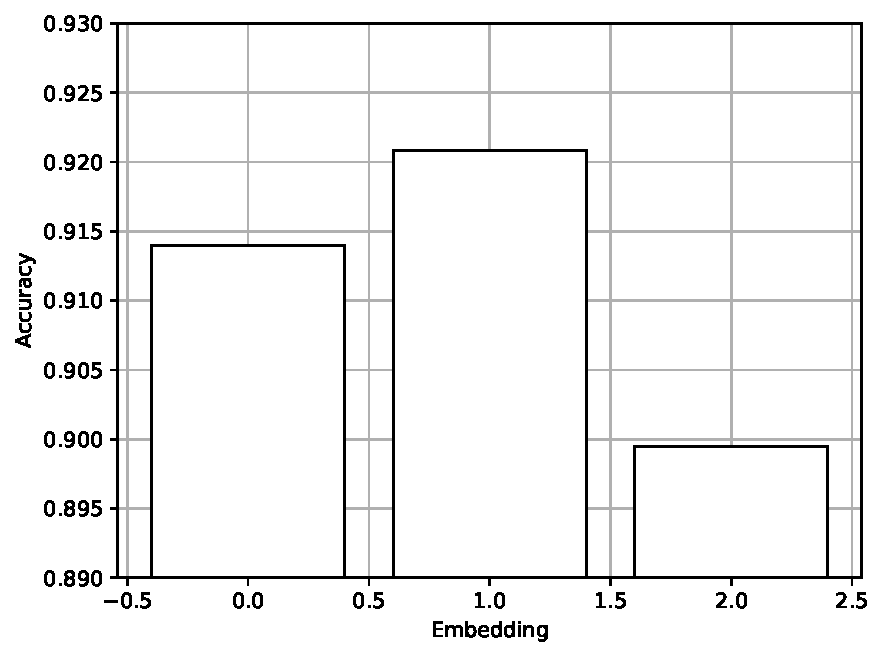
\includegraphics[width=0.8\linewidth]{images/random_graph.pdf}
        \caption{POS-tagging results with random OOV embedding}
        \label{fig:postag_random_results}
      \end{figure}

      In order to test the best number of features for each
      OOV handling model, the model and the embedding were set to be
      in evaluation mode or frozen, meaning that the parameters would
      not change when training the POS-tagger model. The OOV embedding
      from both model on top of the pre-trained embedding was used as
      input for POS-tagging task. Firstly, the embedding for OOV
      entries were predicted through the OOV handling model and added
      to the pre-trained word embedding. Then the collection of the
      pre-trained embedding and the predicted OOV embedding weights
      were fixed so it would not be changed in the training process.
      The results of different number of features on different
      pre-trained embeddings are shown in figure
      \ref{fig:postag_word2vec_freeze_results}, figure
      \ref{fig:postag_polyglot_freeze_results}, and figure
      \ref{fig:postag_dict2vec_freeze_results}. With this settings,
      only CNN with 20 number of features can outperforms the
      \textsc{Mimick} model in Word2vec word embedding while
      \textsc{Mimick} performs better in the other word embedding
      across different number of features that was used. Interestingly, this
      setting for both models perform worse than randomly initialized
      OOV embeddings for Dict2vec pre-trained embedding.
      \begin{figure}[H]
        \centering
        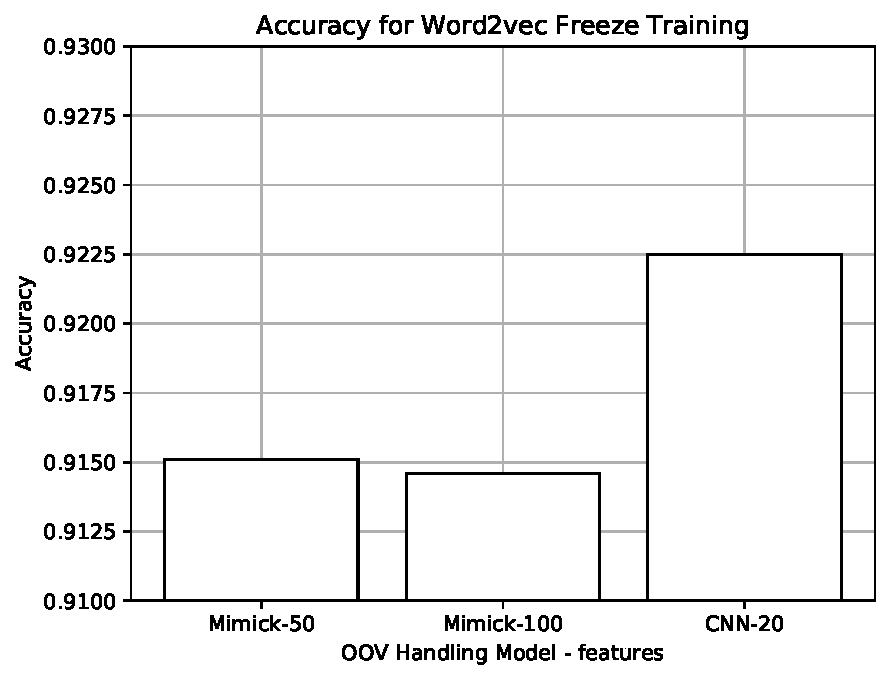
\includegraphics[width=0.8\linewidth]{images/freeze_word2vec.pdf}
        \caption{POS-tagging results frozen embeddings (Word2vec)}
        \label{fig:postag_word2vec_freeze_results}
      \end{figure}
      \begin{figure}[H]
        \centering
        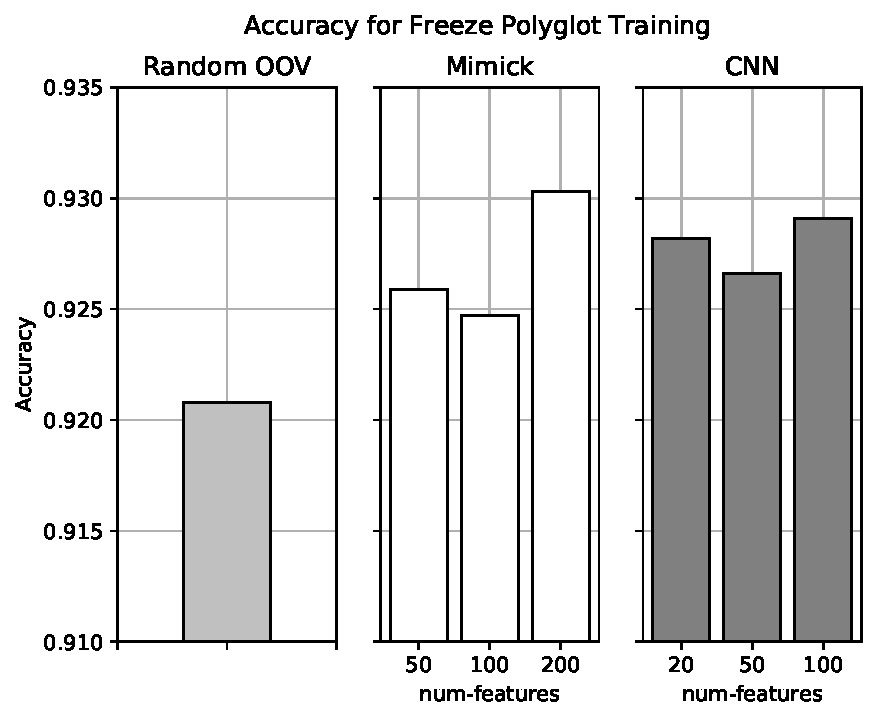
\includegraphics[width=0.8\linewidth]{images/freeze_polyglot.pdf}
        \caption{POS-tagging results frozen embeddings (Polyglot)}
        \label{fig:postag_polyglot_freeze_results}
      \end{figure}
      \begin{figure}[H]
        \centering
        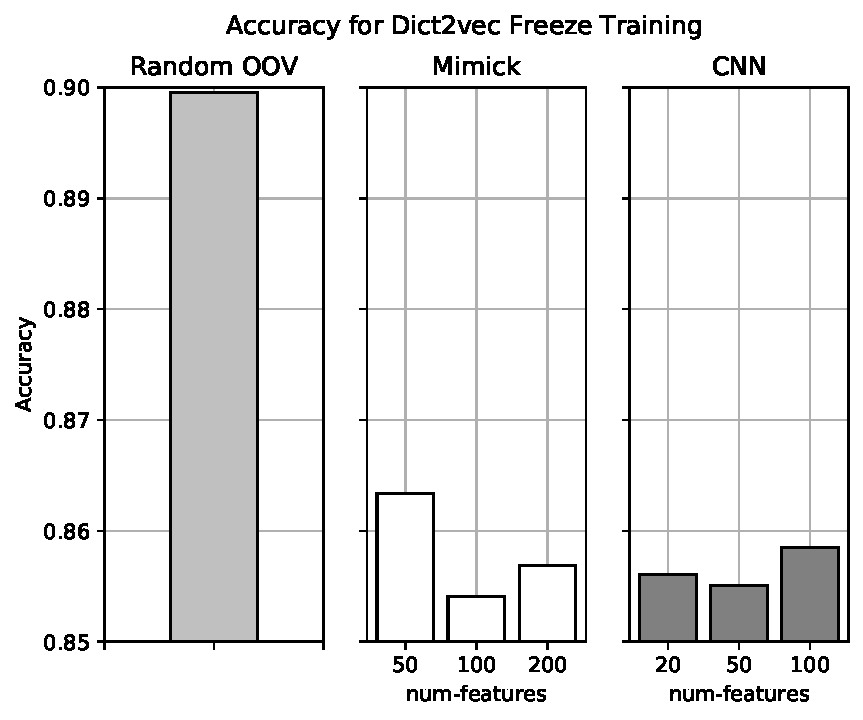
\includegraphics[width=0.8\linewidth]{images/freeze_dict2vec.pdf}
        \caption{POS-tagging results frozen embeddings (Dict2vec)}
        \label{fig:postag_dict2vec_freeze_results}
      \end{figure}
      
      Secondly, the OOV handling model was also trained in conjunction
      with the POS-tagger to improve accuracies of the POS-tagger as
      well as to see whether further improvement in accuracy can
      be achieved by training both the OOV handling model and the
      POS-tagger. Note that the word embedding parameters was still
      untrainable in this setting. The results of these experiments
      are shown in figure
      \ref{fig:postag_word2vec_continuous_results}, figure
      \ref{fig:postag_polyglot_continuous_results}, and figure
      \ref{fig:postag_dict2vec_continuous_results}. The accuracy was
      increased for both OOV handling model as expected surpassing the
      randomly initialized OOV embeddings and the previous setting
      across all pre-trained embeddings. Surprisingly, by allowing the
      OOV handling model to be trained the accuracies of the
      POS-tagger model that used CNN as the OOV handling model were
      surpassing the accuracies from POS-tagger that used
      \textsc{Mimick} as the OOV handling model in all of the
      pre-trained embeddings used in this research.
      \begin{figure}[H]
        \centering
        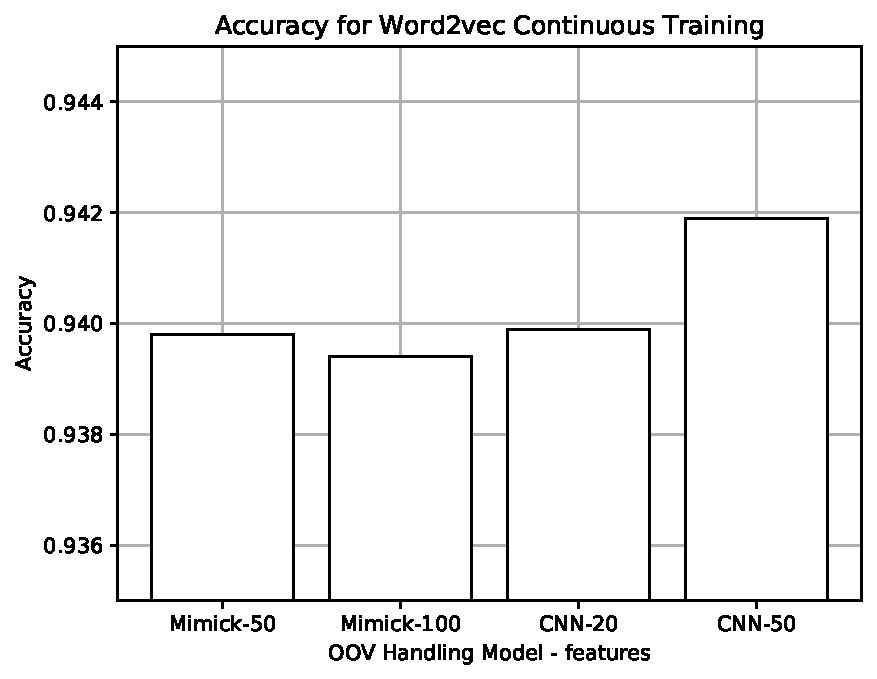
\includegraphics[width=0.8\linewidth]{images/continuous_word2vec.pdf}
        \caption{POS-tagging results continuous embeddings (Word2vec)}
        \label{fig:postag_word2vec_continuous_results}
      \end{figure}
      \begin{figure}[H]
        \centering
        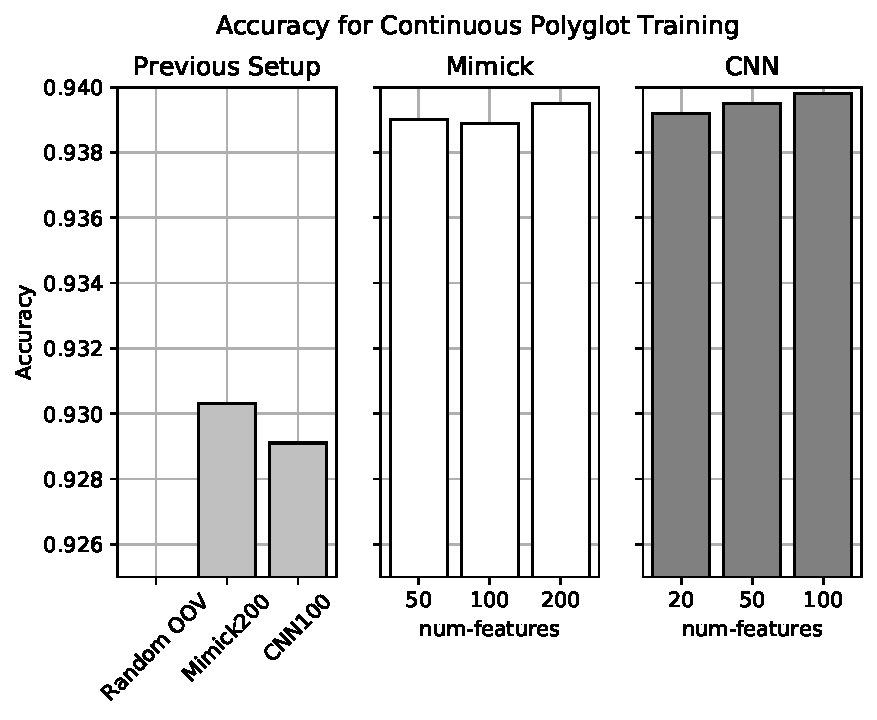
\includegraphics[width=0.8\linewidth]{images/continuous_polyglot.pdf}
        \caption{POS-tagging results continuous embeddings (Polyglot)}
        \label{fig:postag_polyglot_continuous_results}
      \end{figure}
      \begin{figure}[H]
        \centering
        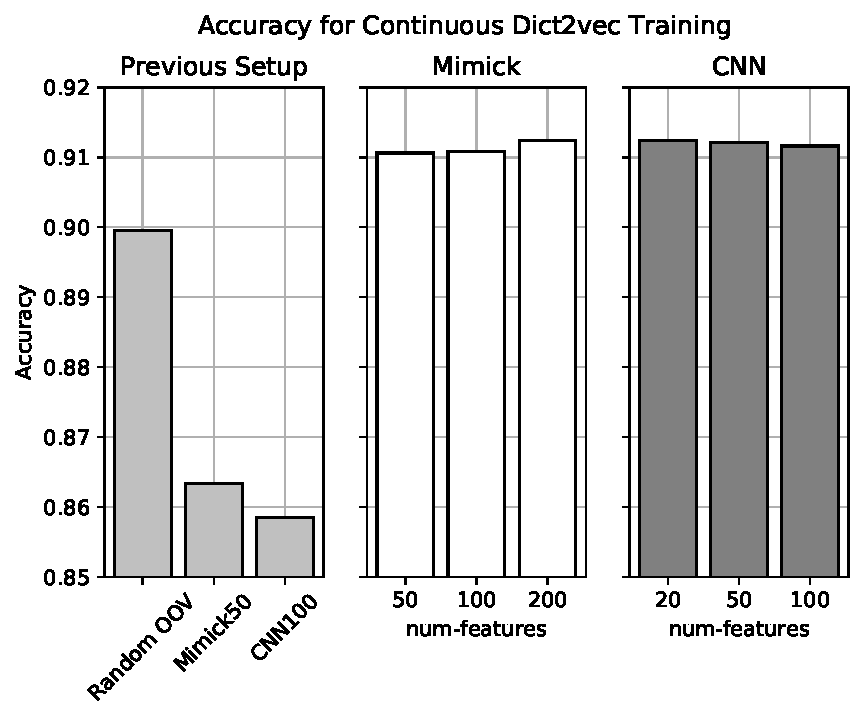
\includegraphics[width=0.8\linewidth]{images/continuous_dict2vec.pdf}
        \caption{POS-tagging results continuous embeddings (Dict2vec)}
        \label{fig:postag_dict2vec_continuous_results}
      \end{figure}

      Thirdly, to simulate how such model will be used in the
      downstream tasks application, both the pre-trained embedding and
      the OOV handling model would be trained and the results were
      compared to previously stated testing method. The number of
      features with the highest results from each OOV handling model
      for each word embedding from the second method were used for the
      current method. The results are shown in figure
      \ref{fig:postag_train_embed_results}. For this setting, CNN
      model were able to outperform \textsc{Mimick} for Polyglot and
      Dict2vec embeddings while it performed worse for Word2vec
      embedding.
      \begin{figure}[H]
        \centering
        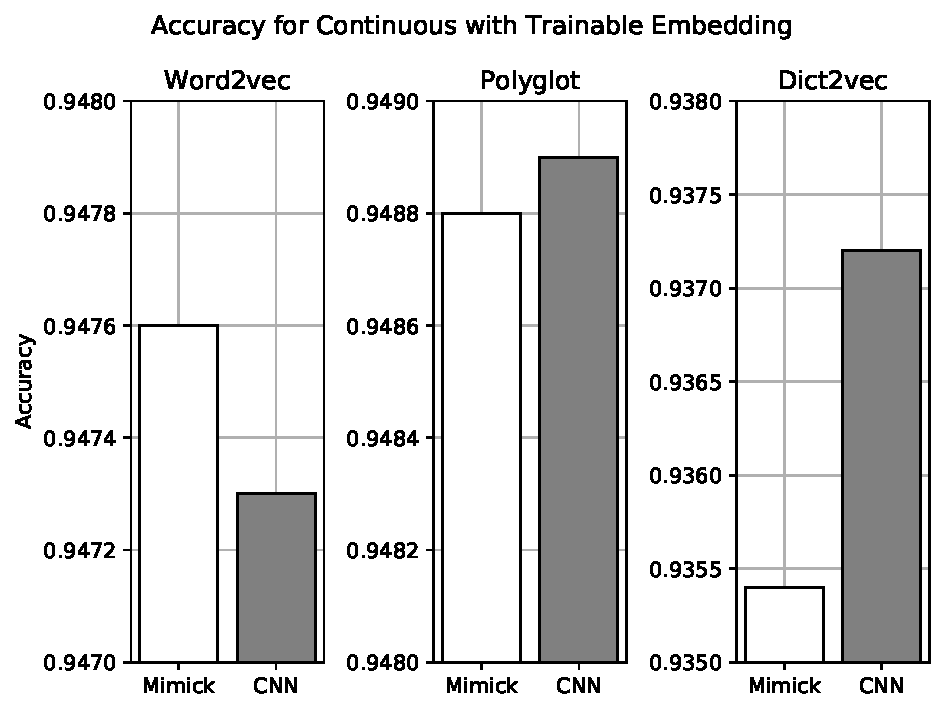
\includegraphics[width=0.8\linewidth]{images/train_embed.pdf}
        \caption{POS-tagging results for OOV handling model and pre-trained embeddings training}
        \label{fig:postag_train_embed_results}
      \end{figure}
      
      Given the results from various settings, in general CNN was
      able to achieve higher accuracies for Brown tag-set dataset.
      Even though \textsc{Mimick} is better at predicting OOV
      embeddings for downstream tasks right \textit{out-of-the-box},
      CNN still outperform \textsc{Mimick} when the OOV handling model
      was also included in the training. This proofs that CNN are able
      to learn OOV handling better for POS-tagging tasks compared to
      bi-LSTM that was used in \textsc{Mimick}.

    \section{Word Similarity}
    For word similarity task, the cosine distance between each given
    pairs from the dataset were calculated. Afterwards, Spearman's rank
    correlation coefficient between the predicted embedding cosine
    distance and the score from the dataset were calculated.

    \begin{table}[!ht]
      \begin{threeparttable} 
      \begin{center}
        \caption{Word Similarity Task Results (word2vec)}
        ~\\
        \label{tab:wordsim:word2vec}
        \begin{tabular}{l|c|c|c|c|c}
          \textbf{Dataset} & \textbf{OOV} & \textbf{Invocab} & \textbf{OOV Ratio} & \textbf{Mimick}\tnote{*} & \textbf{CNN}\tnote{*}\\
          \hline
          card & 989 & 317 & 75.73\% & \textbf{52.27} & 27.25\\
          mc30 & 4 & 35 & 10.26\% & 748.11 & \textbf{758.79}\\
          men & 83 & 668 & 11.05\% & \textbf{672.54} & 664.64\\
          mturk287 & 97 & 402 & 19.44\% & 518.15 & \textbf{519.76}\\
          mturk771 & 18 & 1095 & 1.62\% & \textbf{657.93} & 657.04\\
          rg65 & 2 & 46 & 4.17\% & 709.77 & \textbf{732.61}\\
          rwstanford & 1494 & 1457 & 50.63\% & \textbf{233.83} & 217.47\\
          simlex & 20 & 1008 & 1.95\% & 422.77 & \textbf{425.90}\\
          simverb & 90 & 737 & 10.88\% & \textbf{302.37} & 292.91\\
          verb143 & 4 & 113 & 3.42\% & 467.60 & \textbf{478.25}\\
          wordsim & 15 & 422 & 3.43\% & \textbf{658.92} & 648.25\\
          yp130 & 6 & 141 & 4.08\% & \textbf{460.32} & 443.22\\
          \hline
          \multicolumn{4}{r|}{\textbf{average}} & \textbf{492.05} & 488.84\\
        \end{tabular}
        \begin{tablenotes}
          \item[*] multiplied by 1000
        \end{tablenotes}
      \end{center}
      
    \end{threeparttable} 
    \end{table}
    On the table \ref{tab:wordsim:word2vec}, the OOV handling model
    was trained with Word2vec \citep{Distributed2013mikolov}. The
    predicted embedding from the OOV handling model with highest
    accuracy from POS-tagging tasks were used for calculating the
    Spearman's rank correlation $\rho$. For easier reading, $\rho$
    values are multiplied by 1000. From 12 word similarity datasets,
    CNN model has higher Spearman's rank correlation coefficient on 5
    datasets from 12 datasets with the average Spearman's rank
    correlation coefficient $488.84$ compared to \textsc{Mimick}
    that achieved $492.05$. The highest $\rho$ value for each model
    and each dataset is marked with bold type setting in the table.

    \begin{table}[!ht]
      \begin{threeparttable} 
      \begin{center}
        \caption{Word Similarity Task Results (polyglot)}
        ~\\
        \label{tab:wordsim:polyglot}
        \begin{tabular}{l|c|c|c|c|c}
          \textbf{Dataset} & \textbf{OOV} & \textbf{Invocab} & \textbf{OOV Ratio} & \textbf{Mimick}\tnote{*} & \textbf{CNN}\tnote{*}\\
          \hline
          card & 864 & 442 & 66.16\% & \textbf{128.93} & 114.11\\
          mc30 & 1 & 38 & 2.56\% & 605.25 & 605.25\\
          men & 14 & 737 & 1.86\% & 490.57 & \textbf{492.17}\\
          mturk287 & 76 & 423 & 15.23\% & 443.31 & \textbf{458.81}\\
          mturk771 & 3 & 1110 & 0.27\% & \textbf{432.48} & 432.20\\
          rg65 & 1 & 47 & 2.08\% & 531.59 & \textbf{524.77}\\
          rwstanford & 999 & 1952 & 33.85\% & 272.33 & \textbf{290.78}\\
          simlex & 4 & 1024 & 0.39\% & 232.20 & \textbf{234.16}\\
          simverb & 53 & 774 & 6.41\% & \textbf{137.01} & 134.42\\
          verb143 & 0 & 117 & 0.00\% & 335.81 & 335.81\\
          wordsim & 0 & 437 & 0.00\% & 412.83 & 412.83\\
          yp130 & 5 & 142 & 3.40\% & \textbf{44.76} & 44.62\\
          \hline
          \multicolumn{4}{r|}{average} & 338.92 & \textbf{339.99}\\
        \end{tabular}
        \begin{tablenotes}
          \item[*] multiplied by 1000
        \end{tablenotes}
      \end{center}
    \end{threeparttable} 
    \end{table}

    The same procedure was used for both models was that trained with
    polyglot \citep{polyglot2013alrfou}. From 12 word similarity
    datasets, \textsc{Mimick} has 4 datasets that has higher
    Spearman's rank correlation coefficient than CNN model and 5
    datasets that is lower compared to CNN model while the other 2 has
    similar $\rho$ value because of no OOV entries. In contrast with
    the model trained with word2vec, the model trained with polyglot
    \citep{polyglot2013alrfou} only achieved Spearman's rank
    correlation coefficient as high as $338.92$ while CNN achieved $339.99$,
    showing that CNN has higher
    $\rho$ value compared to \textsc{Mimick} as shown on Table
    \ref{tab:wordsim:polyglot}.

    \begin{table}[!ht]
      \begin{threeparttable} 
      \begin{center}
        \caption{Word Similarity Task Results (Dict2vec)}
        ~\\
        \label{tab:wordsim:dict2vec}
        \begin{tabular}{l|c|c|c|c|c|c}
          \textbf{Dataset} & \textbf{OOV} & \textbf{Invocab} &
          \textbf{OOV Ratio} & \textbf{Random}\tnote{*} &
          \textbf{Mimick}\tnote{*} & \textbf{CNN}\tnote{*}\\
          \hline
          card & 828 & 478 & 63.40\% & 48.07 & 80.89 & \textbf{95.32}\\
          mc30 & 0 & 39 & 0.00\% & 847.57 & 847.57 & 847.57\\
          men & 1 & 750 & 0.13\% & 713.16 & 723.63 & \textbf{723.89}\\
          mturk287 & 2 & 497 & 0.40\% & 652.27 & \textbf{655.32} & 653.13\\
          mturk771 & 0 & 1113 & 0.00\% & 683.91 & 683.91 & 683.91\\
          rg65 & 0 & 48 & 0.00\% & 832.86 & 832.86 & 832.86\\
          rwstanford & 619 & 2332 & 20.98\% & 214.60 & \textbf{403.79} & 400.27\\
          simlex & 3 & 1025 & 0.29\% & 454.80 & \textbf{460.66} & 459.87\\
          simverb & 24 & 803 & 2.90\% & 375.15 & 390.09 & \textbf{393.39}\\
          verb143 & 0 & 117 & 0.00\% & 187.82 & 187.82 & 187.82\\
          wordsim & 18 & 419 & 4.12\% & 642.71 & 718.72 & \textbf{723.72}\\
          yp130 & 2 & 145 & 1.36\% & 577.76 & 621.38 & \textbf{621.75}\\
          \hline
          \multicolumn{4}{r|}{average} & 519.22 & 550.55 & \textbf{551.96}\\
        \end{tabular}
        \begin{tablenotes}
          \item[*] multiplied by 1000
        \end{tablenotes}
      \end{center}
    \end{threeparttable} 
    \end{table}

    For the baseline embedding Dict2vec \citep{dict2vect2017tissier},
    the original embedding was added with randomly generated embedding
    for OOV. The one with highest results from five random seed for
    each dataset was selected. Afterwards, the results was compared
    with CNN and \textsc{Mimick} models. Dict2vec with random OOV
    embedding was only able to achieve Spearman's rank correlation
    coefficient of $519.22$ while \textsc{Mimick} model and CNN model
    were able to achieve $550.55$ and $551.96$ on average respectively
    as shown on Table \ref{tab:wordsim:dict2vec}. This shows that both
    OOV handling models can handle OOV better than initializing
    embedding randomly for OOV for word similarity tasks, especially
    when there is OOV entries. On top of that, for Dict2vec word
    embedding CNN performs better than \textsc{Mimick} in many datasets.

    In summary, for word similarity tasks over 12 datasets and 3
    pre-trained word embeddings CNN performs better on Polyglot and
    Dict2vec while \textsc{Mimick} performs better on word2vec in word
    similarities tasks. This further proved that CNN are better for
    handling OOV than \textsc{Mimick}.

%-----------------------------------------------------
% Chapter: Conclusion
%-----------------------------------------------------
\chapter{Conclusion}
\label{chap:conc}

I was right all along.

\section{What was I right about?}

I was right about the following things.

\subsection{Previous theories were wrong}

People thought they understood, but they didn't.

\subsection{My new idea is right}

Of course.


%%%%%%%%%%%%%%%%%%%%%%%%%%%%
% BIBLIOGRAPHY
\clearpage
\phantomsection
\addcontentsline{toc}{chapter}{Bibliography}
\bibliography{bibli}
%%%%%%%%%%%%%%%%%%%%%%%%%%%%


%%%%%%%%%%%%%%%%%%%%%%%%%%%%
% START APPENDICES
\appendix
%%%%%%%%%%%%%%%%%%%%%%%%%%%%


%-----------------------------------------------------
% Appendix: Code
%-----------------------------------------------------
\chapter{Code}
\label{app:code}

\begin{verbatim}
10 PRINT "HELLO WORLD"
\end{verbatim}


%%%%%%%%%%%%%%%%%%%%%%%%%%%%
% END DOCUMENT
\end{document}
%%%%%%%%%%%%%%%%%%%%%%%%%%%%